\documentclass{article}


\usepackage{anysize} 
\usepackage{amsfonts}
\usepackage{amssymb}
\usepackage{amsmath}
\usepackage{mathrsfs}
\usepackage{amsthm}
\usepackage{appendix}
\usepackage{enumerate}
\usepackage{fancyhdr}
\usepackage{mathtools, bm}
\usepackage[french]{babel}
\selectlanguage{french}
\usepackage[T1]{fontenc}
\usepackage[utf8]{inputenc}
\usepackage{color}
\usepackage{dsfont}

\pagestyle{fancy}
\renewcommand\headrulewidth{1pt}
\fancyhead[L]{Thibaut LANNERS}
\fancyhead[R]{Modélisation Stochastique}

\fancyfoot[R]{15 novembre 2021}

\marginsize{2cm}{2cm}{1.5cm}{1.5cm}

\newtheoremstyle{exostyle}{\topsep}{\topsep}{}{}{\bfseries}{ }{ }{\thmname{#1}\thmnote{. \normalfont{\textit{#3}}}}


\theoremstyle{exostyle}
\newtheorem{exercice}{}

\newenvironment{questions}{
\begin{enumerate}[\hspace{12pt} 1.]}{\end{enumerate}} 

\newtheorem*{prop}{Proposition}
\newtheorem*{preuve}{Preuve}

\begin{document}

\begin{center} 
	{\large\bf{Méthodes de Monte Carlo et techniques de réduction de variance. Application au pricing d'options.}}
\end{center}

\bigskip

\bigbreak
\bigbreak
\bigbreak
\bigbreak
\bigbreak
\bigbreak

\renewcommand{\contentsname}{Sommaire}
\tableofcontents




\newpage



\section{Modèle étudié et problématiques}

\noindent Le but de ce projet est d'estimer le prix des options de type européen à l'instant $t=0$ par la méthode de Monte Carlo et d'implémenter plusieurs méthodes de réduction de variance.\\ Au total nous allons voir $4$ méthodes de Monte Carlo différentes et il faudra décider laquelle est la meilleure en comparant divers facteurs (variance, vitesse de convergence...).\\

\noindent On note $C$ (resp.$P$) le prix de l'option d'achat (resp. de vente), à l'instant $t=0$, c'est la prime. Ce sont donc $C$ et $P$ que l'on cherche à estimer dans ce projet : cela s'appelle le \textbf{pricing d'options}.\\

\noindent Les méthodes de Monte Carlo font parties des outils qui permettent de faire du pricing d'options, mais il va falloir nous intéresser également à la précision de ces méthodes pour juger s'il est intéressant ou non de les employer.\\

\noindent Pour répondre à ces problématiques, on se basera sur la formule de Black-Scholes : 

\[C = \mathbb{E}[(\text{exp}(\beta G) - K)_{+}],\]

\noindent où $G$ est une variable aléatoire gaussienne centrée et réduite, $\beta > 1$, et $K$ est le prix d'exercice.\\

\noindent On a aussi : 

\[P = \mathbb{E}[(K - \text{exp}(\beta G) )_{+}].\]

\bigbreak

\noindent Dans les sections qui vont suivre, on choisira toujours un intervalle de confiance au niveau $95 \%$ pour nos méthodes de Monte-Carlo.







\section{Pricing des options européennes}

\subsection{Formule de Black-Scholes}

\begin{exercice}

\begin{questions}

\bigbreak

\item Montrons que 

\[C = \text{e}^\frac{\beta^{2}}{2}N\left(\beta-\frac{\text{log(K)}}{\beta}\right)-KN\left(-\frac{\text{log}(K)}{\beta}\right),\]

avec $N(x) = \mathbb{P}(G \leq x) = \int_{-\infty}^{x}\frac{\text{e}^{-\frac{y^{2}}{2}}}{\sqrt{2\pi}}dy$ $\forall x \in \mathbb{R}$, où $G$ est une variable aléatoire gaussienne centrée réduite. Autrement dit, $N$ est la fonction de répartition de $G$.

\bigbreak
\bigbreak

Avant de montrer ce résultat, voyons la proposition suivante qui nous sera utile pour la suite.
\begin{prop}
Soit $G$ une variable aléatoire gaussienne centrée réduite et $N$ la fonction de répartition de $G$ comme définie dans l'énoncé (et juste au-dessus également). Soit $\phi(x) = \int_{x}^{\infty}\frac{\text{e}^{-\frac{y^{2}}{2}}}{\sqrt{2\pi}}dy$, $\forall x \in \mathbb{R}$. On a alors les deux égalités suivantes : $\forall x \in \mathbb{R}$,

\[\left\{
  \begin{array}{lll}
    N(-x) = 1 - N(x) \hspace{1cm} (1)\\
    N(x) + \phi(x) = 1 \hspace{1.406cm} (2)
    \end{array}
\right.\]

\end{prop}

\bigbreak

\begin{preuve} Soit $x \in \mathbb{R}$.\\

\underline{Pour (1) :} 

\begin{align*}
    N(x) &= \mathbb{P}(G \leq x)\\
    &= 1-\mathbb{P}(G \geq x)\\
    \leftbrace{\text{Car $G \sim \mathcal{N}(0,1)$} \rightarrow}&= 1-\mathbb{P}(G \leq -x)\\
    &= 1-N(-x).
\end{align*}   

Et donc on a bien $N(-x) = 1-N(x)$.\\
\\
\underline{Pour (2) :}

\begin{align*}
    N(x) + \phi(x) &= \mathbb{P}(G \leq x) + \mathbb{P}(G \geq x)\\
    &= 1 - \mathbb{P}(G \geq x) + \mathbb{P}(G \geq x)\\
    &= 1.
\end{align*} \hspace{15.75cm} \qedsymbol
\end{preuve}


\bigbreak
\bigbreak
\bigbreak

Pour toute la section 2.1, on note $G$ une variable aléatoire gaussienne centrée réduite.\\

\\

On a $C = \mathbb{E}[(\text{exp}(\beta G)-K)_{+}]$.

\bigbreak

Donc en appliquant le théorème de transfert,
\[C = \int_{\mathbb{R}} (\text{exp}(\beta x) - K)_{+} \times \frac{e^{-\frac{x^{2}}{2}}}{\sqrt{2\pi}}dx.\]

On a :

\begin{align*}
    \text{exp}(\beta x)-K \ \geq \ 0 \ &\Leftrightarrow \  \beta x \geq \text{ln}(K)\\
    &\Leftrightarrow \ x \ \geq \ \frac{\text{ln}(K)}{\beta} \ \ \text{car $\beta \ > \ 0$.}
\end{align*}

Ainsi, 

\begin{align*}
    C &= \int_{\frac{\text{ln}(K)}{\beta}}^{+\infty} \text{exp}((\beta x)-K) \frac{e^{-\frac{x^{2}}{2}}}{\sqrt{2\pi}}dx\\
    &= \frac{1}{\sqrt{2\pi}} \int_{\frac{\text{ln}(K)}{\beta}}^{+\infty} \left[ \text{exp}\left( \beta x - \frac{x^{2}}{2} \right) - K \text{e}^{-\frac{x^{2}}{2}}\right]dx\\
    &= \frac{1}{\sqrt{2\pi}} \int_{\frac{\text{ln}(K)}{\beta}}^{+\infty} \text{exp}\left( \beta x - \frac{x^{2}}{2} \right)dx - \frac{1}{\sqrt{2\pi}} \int_{\frac{\text{ln}(K)}{\beta}}^{+\infty} K \text{e}^{-\frac{x^{2}}{2}}dx.\\
\end{align*}

Posons : 

\[\left\{
  \begin{array}{lll}
    I_{1} := \int_{\frac{\text{ln}(K)}{\beta}}^{+\infty} \frac{K \text{e}^{-\frac{x^{2}}{2}}}{\sqrt{2\pi}}dx\\
    I_{2} := \int_{\frac{\text{ln}(K)}{\beta}}^{+\infty} \frac{1}{\sqrt{2\pi}} \text{exp}\left( \beta x - \frac{x^{2}}{2} \right)dx,
\end{array}
\right.\]

de tel sorte qu'on ait : $C = I_{2}-I_{1}$.\\
\\

Tout d'abord, on remarque que $\int_{\frac{\text{ln}(K)}{\beta}}^{+\infty} \frac{ \text{e}^{-\frac{x^{2}}{2}}}{\sqrt{2\pi}}dx = \mathbb{P}\left(G \geq \frac{\text{ln}(K)}{\beta} \right)$.\\
On a donc : 

\begin{align*}
    I_{1} &= \int_{\frac{\text{ln}(K)}{\beta}}^{+\infty} \frac{K \text{e}^{-\frac{x^{2}}{2}}}{\sqrt{2\pi}}dx\\
    &= K \mathbb{P}\left(G \geq \frac{\text{ln}(K)}{\beta} \right)\\
    &= K \left( 1 - \mathbb{P}\left(G \leq \frac{\text{ln}(K)}{\beta} \right)\right)\\
    \leftbrace{\text{Par définition de $N$} \rightarrow} &= K\left( 1 - N\left( \frac{\text{ln}(K)}{\beta} \right) \right)\\
    \leftbrace{\text{D'après (1)} \rightarrow} &= KN\left( -\frac{\text{ln}(K)}{\beta} \right).
\end{align*}

\bigbreak
\bigbreak

On s'intéresse à présent au calcul de $I_{2}$.
En utilisant une identité remarquable de type $(a-b)^{2}$, on a :

\[I_{2} = \int_{\frac{\text{ln}(K)}{\beta}}^{+\infty} \frac{1}{\sqrt{2\pi}}\text{exp}\left(-\frac{1}{2}(x-\beta)^{2}+\frac{\beta^{2}}{2} \right)dx.\]

On fait un changement de variable : on pose $y = x-\beta$, donc $dy=dx$.\\
\\
Donc, 

\begin{align*}
    I_{2} &= \int_{\frac{\text{ln}(K)}{\beta}-\beta}^{+\infty} \frac{1}{\sqrt{2\pi}}\text{exp}\left( -\frac{1}{2}y^{2}\right) \text{exp}\left( \frac{\beta^{2}}{2}\right)dy\\
    &= \text{exp}\left( \frac{\beta^{2}}{2}\right) \underbrace{\int_{\frac{\text{ln}(K)}{\beta}-\beta}^{+\infty} \frac{1}{\sqrt{2\pi}}\text{exp}\left( -\frac{1}{2}y^{2}\right)dy}_{= \mathbb{P}\left(G \geq \frac{\text{ln}(K)}{\beta} - \beta \right)}\\
    &= \text{exp}\left( \frac{\beta^{2}}{2}\right) \left( 1 - \mathbb{P}\left(G \leq \frac{\text{ln}(K)}{\beta} - \beta \right)\right)\\
    &= \text{exp}\left( \frac{\beta^{2}}{2}\right) \left( 1-N\left( \frac{\text{ln}(K)}{\beta} - \beta \right) \right)\\
    \leftbrace{\text{D'après (1)} \rightarrow} &= \text{exp}\left( \frac{\beta^{2}}{2}\right) N\left( \beta - \frac{\text{ln}(K)}{\beta} \right).
\end{align*}

Finalement, on a : 

\hspace{3.4cm}\fcolorbox{red}{white}{$C = I_{2} - I_{1} = -KN \left( -\frac{\text{ln}(K)}{\beta} \right) + \text{exp}\left( \frac{\beta^{2}}{2}\right)N\left( \beta - \frac{\text{ln}(K)}{\beta}\right).$}

\bigbreak
\bigbreak


\item Montrons que

\[P = KN\left( \frac{\text{log}(K)}{\beta}\right) - \text{e}^{\frac{\beta^{2}}{2}}N\left( \frac{\text{log}(K)}{\beta} - \beta\right).\]

On a $P = \mathbb{E}[(K-\text{exp}(\beta G))_{+}]$.

Donc en appliquant le théorème de transfert,

\[P = \int_{\mathbb{R}} (K-\text{exp}(\beta x))_{+} \times \frac{\text{e}^{-\frac{x^{2}}{2}}}{\sqrt{2\pi}}dx.\]


On a :

\begin{align*}
    K - \text{exp}(\beta x) \ \geq \ 0 \ &\Leftrightarrow \ \text{exp}(\beta x) \  \leq \ K\\
    &\Leftrightarrow \ \beta x \ \leq \ \text{ln}(K)\\
    &\Leftrightarrow \ x \ \leq \ \frac{\text{ln}(K)}{\beta} \ \ \ \ \text{car $\beta > 0$.}
\end{align*}


Ainsi, 

\begin{align*}
    P &= \int_{-\infty}^{\frac{\text{ln}(K)}{\beta}} (K-\text{exp}((\beta x)) \frac{e^{-\frac{x^{2}}{2}}}{\sqrt{2\pi}}dx\\
    &= \frac{1}{\sqrt{2\pi}} \int_{-\infty}^{\frac{\text{ln}(K)}{\beta}} \left[ K \text{e}^{-\frac{x^{2}}{2}} - \text{exp} \left( \beta x - \frac{x^{2}}{2} \right) \right]dx.
\end{align*}


Posons : 

\[\left\{
  \begin{array}{lll}
    I_{1} := \int_{-\infty}^{\frac{\text{ln}(K)}{\beta}} \frac{K \text{e}^{-\frac{x^{2}}{2}}}{\sqrt{2\pi}}dx\\
    I_{2} := \int_{-\infty}^{\frac{\text{ln}(K)}{\beta}} \frac{1}{\sqrt{2\pi}}\text{exp}\left( \beta x - \frac{x^{2}}{2} \right)dx \ = \ \int_{-\infty}^{\frac{\text{ln}(K)}{\beta}} \frac{1}{\sqrt{2\pi}}\text{exp}\left( - \frac{1}{2} (x-\beta)^{2}+\frac{\beta^{2}}{2} \right)dx,
\end{array}
\right.\]

de tel sorte que $P = I_{1} - I_{2}$.\\
\\

Tout d'abord, on remarque que $\int_{-\infty}^{\frac{\text{ln}(K)}{\beta}} \frac{ \text{e}^{-\frac{x^{2}}{2}}}{\sqrt{2\pi}}dx = N \left( \frac{\text{ln}(K)}{\beta} \right)$.\\
On a donc : 

\begin{align*}
    I_{1} &= \int_{-\infty}^{\frac{\text{ln}(K)}{\beta}} \frac{K \text{e}^{-\frac{x^{2}}{2}}}{\sqrt{2\pi}}dx\\
    &= KN \left( \frac{\text{ln}(K)}{\beta} \right).
\end{align*}

\bigbreak
\bigbreak

On s'intéresse à présent au calcul de $I_{2}$.
En utilisant une identité remarquable de type $(a-b)^{2}$, on a :

\[I_{2} = \int_{-\infty}^{\frac{\text{ln}(K)}{\beta}}\frac{1}{\sqrt{2\pi}}\text{exp}\left(-\frac{1}{2}(x-\beta)^{2}+\frac{\beta^{2}}{2} \right)dx.\]

On fait un changement de variable : on pose $y = x-\beta$, donc $dy=dx$.\\
\\
Donc, 

\begin{align*}
    I_{2} &= \int_{-\infty}^{\frac{\text{ln}(K)}{\beta}-\beta} \frac{1}{\sqrt{2\pi}}\text{exp}\left( -\frac{1}{2}y^{2}\right) \text{exp}\left( \frac{\beta^{2}}{2}\right)dy\\
    &= \text{exp}\left( \frac{\beta^{2}}{2}\right) \int_{-\infty}^{\frac{\text{ln}(K)}{\beta}-\beta} \frac{1}{\sqrt{2\pi}}\text{exp}\left( -\frac{1}{2}y^{2}\right)dy\\
    \leftbrace{\text{Par définition de $N$} \rightarrow} &= \text{exp}\left( \frac{\beta^{2}}{2}\right) N\left( \frac{\text{ln}(K)}{\beta} - \beta \right).
\end{align*}


Finalement, on a : 

\hspace{3.4cm}\fcolorbox{red}{white}{$P = I_{1} - I_{2} = KN \left( \frac{\text{ln}(K)}{\beta} \right) - \text{exp}\left( \frac{\beta^{2}}{2}\right)N\left( \frac{\text{ln}(K)}{\beta} - \beta\right).$}

\bigbreak
\bigbreak

\underline{Remarque :} On aurait pu aussi utiliser la formule de parité pour retrouver $P$.

\bigbreak
\bigbreak


\item On note $\phi(x) = \int_{x}^{\infty}\frac{\text{e}^{-\frac{y^{2}}{2}}}{\sqrt{2\pi}}dy$. D'après la proposition citée page $2$, on a que : \[\phi(x) \underset{\underset{\text{(2)}}{\uparrow}}{=} 1-N(x) \underset{\underset{\text{(1)}}{\uparrow}}{=} N(-x).\]

Ainsi, on a :

\[\left\{
  \begin{array}{lll}
    C = -K\phi \left( \frac{\text{ln}(K)}{\beta} \right) + \text{exp} \left( \frac{\beta^{2}}{2} \right) \phi \left( \frac{\text{ln}(K)}{\beta} - \beta \right)\\
    P = K\phi \left( - \frac{\text{ln}(K)}{\beta} \right) - \text{exp} \left( \frac{\beta^{2}}{2} \right) \phi \left( \beta - \frac{\text{ln}(K)}{\beta} \right).
\end{array}
\right.\]

\end{questions}

\end{exercice}


\bigbreak
\bigbreak
\bigbreak

\hspace{-0.51cm}Pour la suite nous allons considérer $\beta = 1$ et $K = 1$.

\bigbreak

\subsection{Méthode de Monte Carlo}

\begin{questions}

\bigbreak

\item On a $C = \mathbb{E}[(\text{exp}(\beta G)-K)_{+}] =\mathbb{E}[(\text{exp}(G)-1)_{+}]$ car $\beta = 1$ et $K = 1$, avec $G$ une variable aléatoire gaussienne centrée et réduite.\\
Soit $(X_{i})_{i \geq 1}$ une suite de variables aléatoires indépendantes et identiquement distribuées (v.a.i.i.d) de loi normale centrée et réduite. Posons $(Y_{i})_{i \geq 1} := \left(\left(\text{e}^{X_{i}}-1\right)_{+}\right)_{i \geq 1}$.
$(Y_{i})_{i \geq 1}$ est une suite de v.a.i.i.d de même loi que $Y_{1} = \left( \text{e}^{X_{1}}-1 \right)_{+}$ car les $X_{i}$ sont des v.a.i.i.d (de loi normale centrée réduite).\\
\\

On observe que : 

\[\mathbb{E} [Y_{1}] = \mathbb{E} \left[ \left(\text{e}^{X_{1}} - 1 \right)_{+} \right] = C.\]

Ainsi, on introduit naturellement l'estimateur suivant :

\[\hat{I}_{n}^{(C)} = \frac{1}{n} \sum_{i=1}^{n} Y_{i} = \frac{1}{n} \sum_{i=1}^{n} \left( \text{e}^{X_{i}} - 1 \right)_{+},\]

où $n \in \mathbb{N}^{*}$ correspond au nombre de simulations.\\

Commme $\mathbb{E} [\hat{I}_{n}^{(C)}] = \frac{1}{n} \sum_{i=1}^{n} \mathbb{E} \left[ \left(\text{e}^{X_{i}} - 1 \right)_{+}\right] = \frac{1}{n} \times nC = C$, l'estimateur est sans biais.\\
\\

Montrons à présent que les $(Y_{i})_{i \geq 1}$ sont intégrables afin de pouvoir appliquer la loi forte des grands nombres :

On veut donc montrer que $\mathbb{E}[Y_{1}] = C < \infty$. Or, d'après l'exercice 1 - question 1, on a que :
\[C = \text{exp}\left( \frac{\beta^{2}}{2}\right)N\left( \beta - \frac{\text{ln}(K)}{\beta}\right) -KN \left( -\frac{\text{ln}(K)}{\beta} \right) = \text{e}^{\frac{1}{2}} N(1) - N(0) \hspace{1cm} (3)\]

car on est dans le cas où $\beta = K = 1$. Or, $\forall x \in \mathbb{R}$, $0 \leq N(x) \leq 1$ car $N(x) = \mathbb{P} (G \leq x)$. Donc $C < \infty$ et les $(Y_{i})_{i \geq 1}$ sont intégrables.\\
Ainsi, en appliquant la loi forte des grands nombres on déduit : 

\[\underset{n \to \infty}{\text{lim}} \hat{I}_{n}^{(C)} = \underset{n \to \infty}{\text{lim}} \frac{1}{n} \sum_{i=1}^{n} \left( \text{e}^{X_{i}} - 1 \right)_{+} = C \ \ \text{p.s et dans $L^{1}$}.\]

Montrons que les $(Y_{i})_{i \geq 1}$ admettent un moment d'ordre $2$ afin de pouvoir appliquer le théorème central limite (et donc de pouvoir par la suite écrire une méthode de Monte Carlo pour calculer $C$).\\
On montre donc que $\mathbb{E}[Y_{1}^{2}] < + \infty$. En appliquant le théorème de transfert,

\[\mathbb{E}[Y_{1}^{2}] = \mathbb{E} \left[\left( \left( \text{e}^{X_{1}}-1 \right)_{+} \right)^{2} \right] = \int_{\mathbb{R}} \left( \left(\text{e}^{x}-1 \right)_{+} \right)^{2} \times \frac{\text{e}^{-\frac{x^{2}}{2}}}{\sqrt{2\pi}}dx.\]

On a :

\begin{align*}
    \text{e}^{x}-1 \ \geq \ 0 \ &\Leftrightarrow \ \text{e}^{x} \geq 1\\
    &\Leftrightarrow \ x \ \geq \ 0.
\end{align*}

Ainsi, 

\begin{align*}
    \mathbb{E}\left[ Y_{1}^{2} \right] &= \int_{0}^{+\infty} \left(\text{e}^{x}-1\right)^{2} \times \frac{e^{-\frac{x^{2}}{2}}}{\sqrt{2\pi}}dx\\
    &= \int_{0}^{+\infty}  \left(\text{e}^{2x}-2\text{e}^{x}+1\right) \times \frac{e^{-\frac{x^{2}}{2}}}{\sqrt{2\pi}} dx\\
    &= \frac{1}{\sqrt{2\pi}} \int_{0}^{+\infty} \left(\text{e}^{2x-\frac{x^{2}}{2}}-2\text{e}^{x-\frac{x^{2}}{2}}+\text{e}^{-\frac{x^{2}}{2}}\right)dx.\\
    \leftbrace{\text{Identité remarquable de type $(a-b)^{2}$} \rightarrow} &= \frac{1}{\sqrt{2\pi}} \int_{0}^{+\infty} \left( \text{e}^{-\frac{1}{2}\left(x-2\right)^{2}+2}-2\text{e}^{-\frac{1}{2}\left(x-1\right)^{2}+\frac{1}{2}}+\text{e}^{-\frac{x^{2}}{2}}\right)dx\\
    &=\frac{1}{\sqrt{2\pi}} \int_{0}^{+\infty} \left( \text{e}^{2}\text{e}^{-\frac{(x-2)^{2}}{2}} - 2\text{e}^{\frac{1}{2}}\text{e}^{-\frac{(x-1)^{2}}{2}} + \text{e}^{-\frac{x^{2}}{2}}\right)dx.
\end{align*}


Posons : 

\[\left\{
  \begin{array}{lll}
    I_{1} := \int_{0}^{+\infty} \text{e}^{2} \frac{ \text{e}^{-\frac{(x-2)^{2}}{2}}}{\sqrt{2\pi}}dx\\
    I_{2} := \int_{0}^{+\infty} \text{e}^{\frac{1}{2}} \frac{\text{e}^{-\frac{(x-1)^{2}}{2}}}{\sqrt{2\pi}}dx\\
    I_{3} := \int_{0}^{+\infty} \frac{\text{e}^{-\frac{x^{2}}{2}}}{\sqrt{2\pi}}dx,
\end{array}
\right.\]

de tel sorte qu'on ait : $\mathbb{E}\left[ Y_{1}^{2} \right] = I_{1}-2I_{2}+I_{3}$.\\
\\
\begin{itemize}
    \item \underline{Calcul de $I_{1}$ :}\\
    
    On fait un changement de variable : on pose $y:=x-2$, donc $dy=dx$.\\
    \\
Donc, 

\begin{align*}
    I_{1} &= \text{e}^{2} \int_{-2}^{+\infty} \frac{\text{e}^{-\frac{y^{2}}{2}}}{\sqrt{2\pi}}dy\\
    \leftbrace{\text{Par définition de $\phi$} \rightarrow} &= \text{e}^{2} \phi(-2).
\end{align*}

\item \underline{Calcul de $I_{2}$ :}\\

On fait un changement de variable : on pose $y:=x-1$, donc $dy=dx$.\\
    \\
Donc, 

\begin{align*}
    I_{2} &= \text{e}^{\frac{1}{2}} \int_{-1}^{+\infty} \frac{\text{e}^{-\frac{y^{2}}{2}}}{\sqrt{2\pi}}dy\\
    \leftbrace{\text{Par définition de $\phi$} \rightarrow} &= \text{e}^{\frac{1}{2}} \phi(-1).
\end{align*}

\item \underline{Calcul de $I_{3}$ :}\\

Par définition de $\phi$, on a : 

\[I_{3} = \phi(0).\]
\end{itemize}

Finalement, on a : 

\begin{align*}
    \mathbb{E}\left[ Y_{1}^{2} \right] &= I_{1} - 2I_{2} + I_{3}\\
    &= \text{e}^{2} \phi(-2) -2\text{e}^{\frac{1}{2}} \phi(-1) + \phi(0).
\end{align*}

Or, $\forall x \in \mathbb{R}$, $0 \leq \phi(x) \leq 1$ car $\phi(x) = \mathbb{P} (G \geq x)$. Donc $\mathbb{E}\left[ Y_{1}^{2} \right] < \infty$ et les $(Y_{i})_{i \geq 1}$ admettent un moment d'ordre 2.\\

On pose $\sigma^{2} := \text{Var}(Y_{1}) = \mathbb{E}\left[ Y_{1}^{2} \right] - C^{2}$.\\
On a immédiatement :

\[\text{Var}(\hat{I}_{n}^{(C)}) = \frac{\sigma^{2}}{n}.\]

L'application du théorème central limite implique que, lorsque $n$ tend vers l'infini, 

\[\frac{\sqrt{n}}{\sigma}(\hat{I}_{n}^{(C)} - C) \ \ \text{converge en loi vers $\mathcal{N}(0,1)$,}\]

et signifie intuitivement que, pour $n$ très grand, $\hat{I}_{n}^{(C)} - C \approx \frac{\sigma}{\sqrt{n}}G$, où $G$ est une gaussienne centrée réduite. Il est donc naturel d'introduire l'erreur standard $\frac{\sigma}{\sqrt{n}}$ et l'erreur relative $\frac{1}{C}\frac{\sigma}{\sqrt{n}}$.

Ici, la valeur exacte de $C$ est connue (nous allons la déterminer après) et donc la variance $\sigma^{2}$ ne nous est pas inconnue (on la calculera après $C$). Cependant, nous appliquerons l'algorithme de Monte Carlo en  remplaçant $\sigma^{2}$ par l'estimateur classique de la variance : 

\[s_{n}^{2} = \frac{1}{n-1} \sum_{i=1}^{n} \left( Y_{i} - \hat{I}_{n}^{(C)} \right)^{2} = \frac{1}{n-1} \left( \sum_{i=1}^{n} Y_{i}^{2} - n(\hat{I}_{n}^{(C)})^{2} \right).\]

On sait que $s_{n}^{2}$ converge p.s vers $\sigma^{2}$. Pour estimer l'erreur standard et l'erreur relative, on remplace donc $\sigma^{2}$ par $s_{n}^{2}$ :\\
\\
Nous allons donc utiliser les approximations suivantes :\\
\\
\textit{Erreur standard} : $e = \frac{\sigma}{\sqrt{n}} \approx \frac{s_{n}}{\sqrt{n}}$\\
\textit{Erreur relative} : $\frac{1}{C}\frac{\sigma}{\sqrt{n}} \approx \frac{1}{\hat{I}_{n}^{(C)}}\frac{s_{n}}{\sqrt{n}}$.

\bigbreak

On peut maintenant donner des intervalles de confiance pour notre estimation, dans l'utilisation du théorème central limite, on remplace la variance $\sigma^{2}$ par son estimation $s_{n}^{2}$ : 

\[\mathbb{P} \left( \left| \hat{I}_{n}^{(C)} - C \right| \leq \epsilon \right) = \mathbb{P} \left( \frac{\sqrt{n}}{s_{n}} \left| \hat{I}_{n}^{(C)} - C \right| \leq \frac{\sqrt{n}}{s_{n}} \epsilon \right) \approx 2 \Phi \left( \frac{\sqrt{n}}{s_{n}}\epsilon\right)-1,\]

où $\Phi$ est la fonction de répartition d'une loi normale centrée réduite.\\

On décide de choisir un intervalle de confiance au niveau $\alpha = 95 \ \%$. Donc : 

\[2\Phi \left( \frac{\sqrt{n}}{s_{n}}\epsilon\right)-1 = \alpha = 0.95 \Leftrightarrow \Phi \left(\frac{\sqrt{n}}{s_{n}}\epsilon\right) = \frac{\alpha+1}{2} = 0.975,\]

et donc $\frac{\sqrt{n}}{s_{n}}\epsilon = 1.96$, ou encore $\epsilon = 1.96 \frac{s_{n}}{\sqrt{n}}$. L'intervalle de confiance de $C$ au nivau $95 \ \%$ est donc :

\[ \left[ \hat{I}_{n}^{(C)} - 1.96 \frac{s_{n}}{\sqrt{n}}, \hat{I}_{n}^{(C)} + 1.96 \frac{s_{n}}{\sqrt{n}} \right].\]

Avant de passer à l'algorithme de Monte Carlo, calculons la valeur exacte de $C$. D'après (3), on a : 

\[C = \text{e}^{\frac{1}{2}} N(1) - N(0).\]

Or, d'après (1) (dans la proposition page $2$), on a $N(0) = 1 - N(0)$, donc $N(0) = \frac{1}{2}$. Pour la valeur de $N(1)$, on se réfère à la table de la loi normale centrée réduite\footnote{cf. \textbf{Annexe A}} (on aurait pu faire de même pour la valeur de $N(0)$) et on trouve que $N(1) = 0,8413$. On a donc : 

\hspace{5.41cm}\fcolorbox{red}{white}{$C = \text{e}^{\frac{1}{2}} \times 0,8413 - \frac{1}{2} \approx 0,8871$.}

Maintenant qu'on connaît la valeur exacte de $C$, on peut calculer la variance théorique $\sigma^{2} = \text{Var}(Y_{1})$ : 

\begin{align*}
    \sigma^{2} &= \mathbb{E} [Y_{1}^{2}] - C^{2}\\
    &= \text{e}^{2} \phi(-2) -2\text{e}^{\frac{1}{2}} \phi(-1) + \phi(0) - \left( \text{e}^{\frac{1}{2}} \times 0,8413 - \frac{1}{2} \right)^{2}\\
    \leftbrace{\text{$\phi(x) = N(-x)$ et $\phi(0) = \frac{1}{2}$} \rightarrow}&= \text{e}^{2} N(2) -2\text{e}^{\frac{1}{2}} N(1) + \frac{1}{2} - \left( \text{e}^{\frac{1}{2}} \times 0,8413 - \frac{1}{2} \right)^{2}.
\end{align*}

On a vu précédemment que $N(1) = 0,8413$. Pour $N(2)$ on se réfère aussi à la table de la loi normale centrée réduite et on trouve que $N(2) = 0,9772$. On a donc : 

\hspace{2.41cm}\fcolorbox{red}{white}{$\sigma^{2} = \text{e}^{2} \times 0,9772 -2\text{e}^{\frac{1}{2}} \times 0,8413 + \frac{1}{2} - \left( \text{e}^{\frac{1}{2}} \times 0,8413 - \frac{1}{2} \right)^{2} \approx 4,1596$.}


\bigbreak

\underline{\textbf{Algorithme de Monte Carlo :}}\\

On peut écrire un algorithme de Monte Carlo car les hypothèses sont vérifiées (en particulier $\mathbb{E} [Y_{1}^{2} ] < \infty)$. Le code Matlab de l'algorithme de Monte Carlo associé à ce point ainsi que le graphique correspondant et les valeurs que nous renvoie le programme est consultable en \textbf{Annexe B - pages 1, 2 et 3}.\\

J'ai exécuté le programme pour différentes valeurs de $n$ : \\

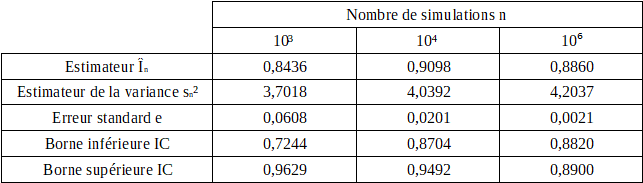
\includegraphics{Tableau_1.PNG}

\bigbreak
\bigbreak

\item On a $P = \mathbb{E} [(K-\text{exp}(\beta G))_{+}] = \mathbb{E}[(1-\text{exp}(G))_{+}]$ car $\beta = 1$ et $K = 1$, avec $G$ une variable aléatoire  gaussienne centrée et réduite.\\
Soit $(X_{i})_{i \geq 1}$ des v.a.i.i.d de loi normale centrée et réduite. Posons $(Y_{i})_{i \geq 1} := \left(\left( 1-\text{e}^{X_{i}}\right)_{+}\right)_{i \geq 1}$.\\
$(Y_{i})_{i \geq 1}$ est une suite de v.a.i.i.d de même loi que $Y_{1} = \left( 1-\text{e}^{X_{1}} \right)_{+}$ car les $X_{i}$ sont des v.a.i.i.d (de loi normale centrée réduite).\\
\\

On observe que : 

\[\mathbb{E} [Y_{1}] = \mathbb{E} \left[ \left(1-\text{e}^{X_{1}} \right)_{+} \right] = P.\]

Ainsi, on introduit naturellement l'estimateur suivant :

\[\hat{I}_{n}^{(P)} = \frac{1}{n} \sum_{i=1}^{n} Y_{i} = \frac{1}{n} \sum_{i=1}^{n} \left( 1-\text{e}^{X_{i}} \right)_{+},\]

où $n \in \mathbb{N}^{*}$ correspond au nombre de simulations.\\

Commme $\mathbb{E} [\hat{I}_{n}^{(P)}] = \frac{1}{n} \sum_{i=1}^{n} \mathbb{E} \left[ \left(1-\text{e}^{X_{i}} \right)_{+}\right] = \frac{1}{n} \times nP = P$, l'estimateur est sans biais.\\
\\

Montrons à présent que les $(Y_{i})_{i \geq 1}$ sont intégrables afin de pouvoir appliquer la loi forte des grands nombres :

On veut donc montrer que $\mathbb{E}[Y_{1}] = P < \infty$. Or, d'après le point $2.$ de la partie $2.1$, on a que :
\[P = KN \left( \frac{\text{ln}(K)}{\beta} \right) - \text{exp}\left( \frac{\beta^{2}}{2}\right)N\left( \frac{\text{ln}(K)}{\beta} - \beta\right) = N(0)-\text{e}^{\frac{1}{2}}N(-1) \hspace{1cm} (4)\]

car on est dans le cas où $\beta = K = 1$. Or, $\forall x \in \mathbb{R}$, $0 \leq N(x) \leq 1$ car $N(x) = \mathbb{P} (G \leq x)$. Donc $P < \infty$ et les $(Y_{i})_{i \geq 1}$ sont intégrables.\\
Ainsi, en appliquant la loi forte des grands nombres on déduit : 

\[\underset{n \to \infty}{\text{lim}} \hat{I}_{n}^{(P)} = \underset{n \to \infty}{\text{lim}} \frac{1}{n} \sum_{i=1}^{n} \left( 1-\text{e}^{X_{i}} \right)_{+} = P \ \ \text{p.s et dans $L^{1}$}.\]

Montrons que les $(Y_{i})_{i \geq 1}$ admettent un moment d'ordre $2$ afin de pouvoir appliquer le théorème central limite.\\
On montre donc que $\mathbb{E}[Y_{1}^{2}] < + \infty$. En appliquant le théorème de transfert,

\[\mathbb{E}[Y_{1}^{2}] = \mathbb{E} \left[\left( \left( 1-\text{e}^{X_{1}} \right)_{+} \right)^{2} \right] = \int_{\mathbb{R}} \left( \left(1-\text{e}^{x} \right)_{+} \right)^{2} \times \frac{\text{e}^{-\frac{x^{2}}{2}}}{\sqrt{2\pi}}dx.\]

On a :

\begin{align*}
    1-\text{e}^{x} \ \geq \ 0 \ &\Leftrightarrow \ \text{exp}^{x} \leq 1\\
    &\Leftrightarrow \ x \ \leq \ 0.
\end{align*}

Ainsi, 

\begin{align*}
    \mathbb{E}\left[ Y_{1}^{2} \right] &= \int_{-\infty}^{0} \left(1-\text{e}^{x}\right)^{2} \times \frac{e^{-\frac{x^{2}}{2}}}{\sqrt{2\pi}}dx\\
    &= \int_{-\infty}^{0}  \left(1-2\text{e}^{x}+\text{e}^{2x}\right) \times \frac{e^{-\frac{x^{2}}{2}}}{\sqrt{2\pi}}dx\\
    \leftbrace{\text{Par analogie au point 1.} \rightarrow} &= \text{e}^{2} N(-2) -2\text{e}^{\frac{1}{2}} N(-1) + N(0)\\
    &< \infty.
\end{align*}

On pose $\sigma^{2} := Var(Y_{1}) = \mathbb{E}\left[ Y_{1}^{2} \right] - P^{2}$.\\
On a immédiatement :

\[\text{Var}(\hat{I}_{n}^{(P)}) = \frac{\sigma^{2}}{n}.\]

L'application du théorème central limite implique que, lorsque $n$ tend vers l'infini, 

\[\frac{\sqrt{n}}{\sigma}(\hat{I}_{n}^{(P)} - P) \ \ \text{converge en loi vers $\mathcal{N}(0,1)$,}\]

et signifie intuitivement que, pour $n$ très grand, $\hat{I}_{n}^{(P)} - P \approx \frac{\sigma}{\sqrt{n}}G$, où $G$ est une gaussienne centrée réduite. Il est donc naturel d'introduire l'erreur standard $\frac{\sigma}{\sqrt{n}}$ et l'erreur relative $\frac{1}{P}\frac{\sigma}{\sqrt{n}}$.

De même que pour le point 1., la valeur exacte de $P$ est connue (nous allons la déterminer après) mais nous allons quand même remplacer $\sigma^{2}$ (qu'on calculera après $P$) par l'estimateur classique de la variance : 

\[s_{n}^{2} = \frac{1}{n-1} \sum_{i=1}^{n} \left( Y_{i} - \hat{I}_{n}^{(P)} \right)^{2} = \frac{1}{n-1} \left( \sum_{i=1}^{n} Y_{i}^{2} - n(\hat{I}_{n}^{(P)})^{2} \right).\]

Nous allons utiliser les approximations suivantes (par anologie au point 1.) :\\
\\
\textit{Erreur standard} : $\frac{\sigma}{\sqrt{n}} \approx \frac{s_{n}}{\sqrt{n}}$\\
\textit{Erreur relative} : $\frac{1}{C}\frac{\sigma}{\sqrt{n}} \approx \frac{1}{\hat{I}_{n}^{(P)}}\frac{s_{n}}{\sqrt{n}}$.\\
\\

Ici, comme pour le point 1., on décide de choisir un intervalle de confiance au niveau $\alpha = 95 \ \%$. Ainsi, l'intervalle de confiance de $P$ au nivau $95 \ \%$ est :

\[ \left[ \hat{I}_{n}^{(P)} - 1.96 \frac{s_{n}}{\sqrt{n}}, \hat{I}_{n}^{(P)} + 1.96 \frac{s_{n}}{\sqrt{n}} \right].\]

Avant de passer à l'algorithme de Monte Carlo, calculons la valeur exacte de $P$. D'après (4), on a : 

\begin{align*}
    P &= N(0) - \text{e}^{\frac{1}{2}} N(-1)\\
    \leftbrace{\text{D'après (1)} \rightarrow} &= N(0) - \text{e}^{\frac{1}{2}} (1-N(1))\\
    \leftbrace{\text{Car $N(0) = \frac{1}{2}$ (montré au point 1.)} \rightarrow} &= \frac{1}{2} - \text{e}^{\frac{1}{2}} + \text{e}^{\frac{1}{2}}N(1)\\
    &= \frac{1}{2} + \text{e}^{\frac{1}{2}} (N(1)-1)\\
   \leftbrace{\text{Car $N(1) = 0,8413$ (cf. \textbf{Annexe A})} \rightarrow} &= \frac{1}{2} + \text{e}^{\frac{1}{2}} (0,8413-1)\\
   &= \frac{1}{2} + \text{e}^{\frac{1}{2}} \times (-0,1587)
\end{align*}

On a donc : 

\hspace{5.1cm}\fcolorbox{red}{white}{$P = \frac{1}{2} + \text{e}^{\frac{1}{2}} \times (-0,1587) \approx 0,2383$.}

\bigbreak

Maintenant qu'on connaît la valeur exacte de $P$, on peut calculer la variance théorique $\sigma^{2} = \text{Var}(Y_{1})$ : 

\begin{align*}
    \sigma^{2} &= \mathbb{E} [Y_{1}^{2}] - P^{2}\\
    &= \text{e}^{2} N(-2) -2\text{e}^{\frac{1}{2}} N(-1) + N(0) - \left(\frac{1}{2} + \text{e}^{\frac{1}{2}} \times (-0,1587)\right)^{2}\\
    \leftbrace{\text{D'après $(1)$ et $N(0) = \frac{1}{2}$} \rightarrow}&= \text{e}^{2} (1-N(2)) -2\text{e}^{\frac{1}{2}} (1-N(1)) + \frac{1}{2} - \left( \frac{1}{2} + \text{e}^{\frac{1}{2}} \times (-0,1587)\right)^{2}.
\end{align*}

Ce qui nous donne, en remplaçant par les valeurs de $N(1)$ et $N(2)$ : 

\hspace{2.41cm}\fcolorbox{red}{white}{$\sigma^{2} = \text{e}^{2} (1 -  0,9772) -2\text{e}^{\frac{1}{2}} (1 - 0,8413) + \frac{1}{2} - \left( \frac{1}{2} + \text{e}^{\frac{1}{2}} \times (-0,1587) \right)^{2} \approx 0,0884$.}

\bigbreak

\underline{\textbf{Algorithme de Monte Carlo :}}\\

On peut écrire un algorithme de Monte Carlo car les hypothèses sont vérifiées (en particulier $\mathbb{E} [Y_{1}^{2} ] < \infty)$. Le code Matlab de l'algorithme de Monte Carlo associé à ce point ainsi que le graphique correspondant et les valeurs que nous renvoie le programme est consultable en \textbf{Annexe B - pages 4, 5 et 6}.\\

J'ai exécuté le programme pour différentes valeurs de $n$ : \\

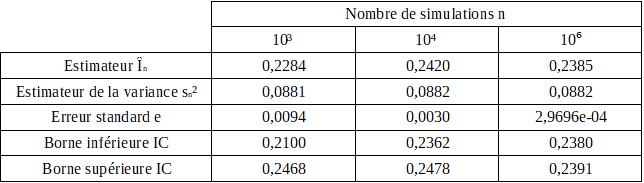
\includegraphics{Tableau_2.PNG}

\bigbreak
\bigbreak

\item Dans les deux cas (pour le call et pour le put), on remarque d'après les deux graphiques que la méthode semble converger à partir d'environ $4000$ simulations. Dans le cas du call, on observe que les variances estimées sont très élevées alors qu'elles sont beaucoup plus faibles dans le cas du put. Ainsi, l'erreur est donc plus élevée pour l'estimation de $C$ que pour celle de $P$. 

\end{questions}

\end{exercice}

\bigbreak
\bigbreak
\bigbreak

\subsection{\'Echantillonnage préférentiel}

\begin{questions}

\bigbreak

\item Soit $Y$ une variable aléatoire exponentielle de paramètre 1. On note $f_{Y}$ la densité de Y, $f_{Y}(x) = \text{e}^{-x} \mathds{1}_{[0,+\infty[}(x)$ $\forall x \in \mathbb{R}$.\\
On a $C = \mathbb{E}[(\text{exp}(G)-1)_{+}]$, avec $G$ une variable aléatoire gaussienne centrée réduite.\\
En appliquant le théorème de transfert,

\[C = \int_{\mathbb{R}} \left( \text{e}^{x}-1 \right)_{+} \frac{1}{\sqrt{2\pi}}\text{e}^{-\frac{x^{2}}{2}}dx.\]

On a :

\begin{align*}
    \text{e}^{x}-1 \ \geq \ 0 \ &\Leftrightarrow \ \text{e}^{x} \geq 1\\
    &\Leftrightarrow \ x \ \geq \ 0.
\end{align*}

Ainsi, 

\[C = \frac{1}{\sqrt{2\pi}} \int_{0}^{+\infty} \left( \text{e}^{x} - 1 \right) \text{e}^{-\frac{x^{2}}{2}}dx.\]

On fait un changement de variable. On pose, $\forall x > 0$ :

\begin{align*}
    & \ \ \ \ \ y = \frac{x^{2}}{2} \ \ (\text{$> 0$})\\
    &\Leftrightarrow x^{2} = 2y\\
    &\Leftrightarrow x = \sqrt{2y} \ \ (\text{car $x > 0$}),
\end{align*}

et $dx = \frac{1}{\sqrt{2y}}dy$.\\
Donc,

\[C = \frac{1}{\sqrt{2\pi}} \int_{0}^{+\infty} \frac{\text{e}^{\sqrt{2y}}-1}{\sqrt{2y}} \text{e}^{-y}dy\]

Regardons si l'intégrale est bien définie en $0$ :


On sait que pour $x$ petit on a $\text{e}^{x}-1 \sim x$. Donc $\frac{\text{e}^{\sqrt{2y}}-1}{\sqrt{2y}} \text{e}^{-y} \underset{y \to 0}{\sim} \text{e}^{-y}$. Ainsi, il n'y a aucun problème en $0$.\\

On a donc : 

\begin{align*}
    C &= \frac{1}{\sqrt{2\pi}} \int_{0}^{+\infty} \frac{\text{e}^{\sqrt{2y}}-1}{\sqrt{2y}} f_{Y}(y)dy\\
    &= \frac{1}{\sqrt{2\pi}} \int_{\mathbb{R}} \frac{\text{e}^{\sqrt{2y}}-1}{\sqrt{2y}} f_{Y}(y) \mathds{1}_{[0,+\infty[}(x)dy\\
    &= \frac{1}{\sqrt{2\pi}} \mathbb{E}\left[ \frac{\text{e}^{\sqrt{2Y}}-1}{\sqrt{2Y}} \right],
\end{align*}
    
où le passage de la deuxième à la troisème ligne est justifié par l'utilisation du théorème de transfert.

\bigbreak
\bigbreak

\item D'après le point 1., on a : 

\[C = \frac{1}{\sqrt{2\pi}} \mathbb{E}\left[ \frac{\text{e}^{\sqrt{2Y}}-1}{\sqrt{2Y}} \right] = \mathbb{E}\left[ \frac{1}{\sqrt{2\pi}} \frac{\text{e}^{\sqrt{2Y}}-1}{\sqrt{2Y}} \right],\]

avec $Y$ une variable aléatoire suivant une loi exponentielle de paramètre $1$.\\
Soit $(Y_{i})_{i \geq 1}$ des v.a.i.i.d de loi exponentielle de paramètre 1. Posons $(Z_{i})_{i \geq 1} := \left( \frac{1}{\sqrt{2\pi}} \frac{\text{e}^{\sqrt{2Y_{i}}}-1}{\sqrt{2Y_{i}}} \right)_{i \geq 1}$.\\
$(Z_{i})_{i \geq 1}$ est une suite de v.a.i.i.d de même loi que $Z_{1} =  \frac{1}{\sqrt{2\pi}} \frac{\text{e}^{\sqrt{2Y_{1}}}-1}{\sqrt{2Y_{1}}}$ car les $Y_{i}$ sont des v.a.i.i.d (de loi exponentielle de paramètre 1).\\
\\

On observe que : 

\[\mathbb{E} [Z_{1}] = \mathbb{E} \left[ \frac{1}{\sqrt{2\pi}} \frac{\text{e}^{\sqrt{2Y_{1}}}-1}{\sqrt{2Y_{1}}} \right] = C.\]

Ainsi, on introduit naturellement l'estimateur suivant :

\[\hat{I}_{n} = \frac{1}{n} \sum_{i=1}^{n} Z_{i} = \frac{1}{n} \sum_{i=1}^{n} \left( \frac{1}{\sqrt{2\pi}} \frac{\text{e}^{\sqrt{2Y_{i}}}-1}{\sqrt{2Y_{i}}} \right),\]

où $n \in \mathbb{N}^{*}$ correspond au nombre de simulations.\\

Commme $\mathbb{E} [\hat{I}_{n}] = \frac{1}{n} \sum_{i=1}^{n} \mathbb{E} \left[ \frac{1}{\sqrt{2\pi}} \frac{\text{e}^{\sqrt{2Y_{i}}}-1}{\sqrt{2Y_{i}}}\right] = \frac{1}{n} \times nC = C$, l'estimateur est sans biais.\\
\\

Les $(Z_{i})_{i \geq 1}$ sont forcéments intégrables car $\mathbb{E}[Z_{1}] = C$ et on a vu dans l'exercice 1 que $C < \infty$. Ainsi, d'après la loi forte des grands nombres on a :

\[\underset{n \to \infty}{\text{lim}} \hat{I}_{n} = \underset{n \to \infty}{\text{lim}} \frac{1}{n} \sum_{i=1}^{n} \left(\frac{1}{\sqrt{2\pi}} \frac{\text{e}^{\sqrt{2Y_{i}}}-1}{\sqrt{2Y_{i}}} \right) = C \ \ \text{p.s et dans $L^{1}$}.\]

Montrons que les $(Z_{i})_{i \geq 1}$ admettent un moment d'ordre $2$ afin de pouvoir appliquer le théorème central limite (Je n'ai pas réussi à le montrer : on le supposera donc).\\

On pose $\sigma^{2} := Var(Z_{1}) = \mathbb{E}\left[ Z_{1}^{2} \right] - C^{2}$.\\
On a immédiatement :

\[\text{Var}(\hat{I}_{n}) = \frac{\sigma^{2}}{n}.\]

L'application du théorème central limite implique que, lorsque $n$ tend vers l'infini, 

\[\frac{\sqrt{n}}{\sigma}(\hat{I}_{n} - C) \ \ \text{converge en loi vers $\mathcal{N}(0,1)$.}\]

De manière analogue à la section 2.1, on procède comme suit.\\
Nous allons remplacer $\sigma^{2}$ par l'estimateur classique de la variance : 

\[s_{n}^{2} = \frac{1}{n-1} \sum_{i=1}^{n} \left( Z_{i} - \hat{I}_{n} \right)^{2} = \frac{1}{n-1} \left( \sum_{i=1}^{n} Z_{i}^{2} - n\hat{I}_{n}^{2} \right).\]

Nous allons utiliser les approximations suivantes :\\

\\
\textit{Erreur standard} : $\frac{\sigma}{\sqrt{n}} \approx \frac{s_{n}}{\sqrt{n}}$\\
\textit{Erreur relative} : $\frac{1}{C}\frac{\sigma}{\sqrt{n}} \approx \frac{1}{\hat{I}_{n}}\frac{s_{n}}{\sqrt{n}}$.

\bigbreak

L'intervalle de confiance de $C$ au nivau $95 \ \%$ est :

\[ \left[ \hat{I}_{n} - 1.96 \frac{s_{n}}{\sqrt{n}}, \hat{I}_{n} + 1.96 \frac{s_{n}}{\sqrt{n}} \right].\]
\\

\underline{\textbf{Algorithme de Monte Carlo :}}\\

On peut écrire un algorithme de Monte Carlo car les hypothèses sont vérifiées (en particulier $\mathbb{E} [Z_{1}^{2} ] < \infty)$. Le code Matlab de l'algorithme de Monte Carlo associé à ce point ainsi que le graphique correspondant et les valeurs que nous renvoie le programme est consultable en \textbf{Annexe C}.\\

J'ai exécuté le programme pour différentes valeurs de $n$ : \\

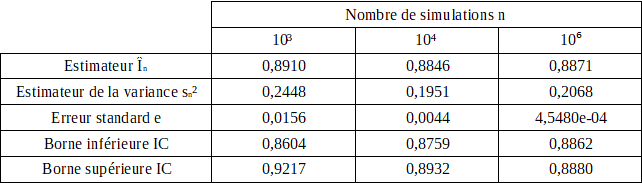
\includegraphics{Tableau_3.PNG}

\bigbreak
\bigbreak

\item Tout d'abord, on sait que la variance de la première méthode (celle de la section $2.1$) est égale à $4,1596$. Or, la variance de la méthode d'échantillonnage préférentiel semble valoir environ $0,2$ en se référant aux trois estimations de la variance obtenue dans notre tableau de résulats présenté à la fin du point 2. ci-dessus. Ainsi, la méthode d'échantillonnage préférentiel est meilleure que la méthode utilisée dans la section 2.1.\\
Cela peut se voir aussi sur les graphes : on remarque tout de suite que la vitesse de convergence de la méthode d'échantillonnage préférentiel est bien plus grande que celle de la première méthode. En effet, on voit (cf. graphe \textbf{Annexe C - page 3}) qu'à partir d'environ $1500$ simulations, la courbe de la valeur approchée de $C$ semble se stabiliser vers la valeur exacte de $C$, contre $4000$ simulations pour la première méthode. 


\end{questions}

\end{exercice}

\bigbreak
\bigbreak
\bigbreak

\subsection{Variables de contrôle}

\begin{questions}

\bigbreak

\item  D'après la section 2.1 (points 1. et 2.), on a (on est toujours dans le cas $\beta=1$ et $K=1$) :

\[\left\{
  \begin{array}{lll}
    C = \text{e}^{\frac{1}{2}}N(1)-N(0)\\
    P = N(0) - \text{e}^{\frac{1}{2}}N(-1).
\end{array}
\right.\]

Donc,

\begin{align*}
    & \ \ \ \ \ C - P = \text{e}^{\frac{1}{2}}N(1)-N(0) - N(0) + \text{e}^{\frac{1}{2}}N(-1)\\
    &\Leftrightarrow C = \text{e}^{\frac{1}{2}}N(1) - 2 \times \frac{1}{2} + \text{e}^{\frac{1}{2}}\left(1-N(1)\right)+P\\
    &\Leftrightarrow C = \text{e}^{\frac{1}{2}} - 1 + P,
\end{align*}

où le passage de la première à la deuxième ligne est justifié par le fait que $N(0) = \frac{1}{2}$ et $N(-1) = 1 - N(1)$ d'après $(1)$.\\

On peut donc estimer $C$ en utilisant une valeur approchée de $P$. On va prendre la valeur de l'estimateur de C obtenu dans la méthode de Monte Carlo du point 2. de la section 2.2 après $10^{6}$ simulations. On avait obtenu : $P \approx 0,2388$.\\

Ainsi, une estimation de $C$ est : 

\[C \approx \text{e}^{\frac{1}{2}} - 1 + 0,2383 \approx 0,8870.\]

\bigbreak
\bigbreak


\item On a vu au point précédent que $C = \text{e}^{\frac{1}{2}} - 1 + P$, et on sait que $P = \mathbb{E} \left[ \left( 1 - \text{e}^{G} \right)_{+} \right]$, avec $G$ une variable aléatoire gaussienne centrée et réduite. On a donc : 

\[C = \text{e}^{\frac{1}{2}} - 1 + \mathbb{E} \left[ \left( 1 - \text{e}^{G} \right)_{+} \right] = \mathbb{E} \left[ \text{e}^{\frac{1}{2}} - 1 + \left( 1 - \text{e}^{G} \right)_{+} \right].\]

Soit $(X_{i})_{i \geq 1}$ une suite de v.a.i.i.d de loi normale centrée réduite. Posons $(Y_{i})_{i \geq 1} := \left( \text{e}^{\frac{1}{2}} - 1 + \left(1-\text{e}^{X_{i}}\right)_{+}\right)_{i \geq 1}$.
$(Y_{i})_{i \geq 1}$ est une suite de v.a.i.i.d de même loi que $Y_{1} = \text{e}^{\frac{1}{2}} - 1 + \left( 1-\text{e}^{X_{1}} \right)_{+}$ car les $X_{i}$ sont des v.a.i.i.d (de loi normale centrée réduite).\\
\\

On observe que : 

\[\mathbb{E} [Y_{1}] = \mathbb{E} \left[ \text{e}^{\frac{1}{2}} - 1 + \left( 1 - \text{e}^{X_{1}} \right)_{+} \right] = C.\]

Ainsi, on introduit naturellement l'estimateur suivant :

\[\hat{I}_{n} = \frac{1}{n} \sum_{i=1}^{n} Y_{i} = \frac{1}{n} \sum_{i=1}^{n} \left( \text{e}^{\frac{1}{2}} - 1 +  \left( 1-\text{e}^{X_{i}} \right)_{+}\right),\]

où $n \in \mathbb{N}^{*}$ correspond au nombre de simulations.\\

Commme $\mathbb{E} [\hat{I}_{n}] = \frac{1}{n} \sum_{i=1}^{n} \mathbb{E} \left[ \text{e}^{\frac{1}{2}} - 1 +  \left(1-\text{e}^{X_{i}} \right)_{+}\right] = \frac{1}{n} \times nC = C$, l'estimateur est sans biais.\\
\\

Montrons à présent que les $(Y_{i})_{i \geq 1}$ sont intégrables afin de pouvoir appliquer la loi forte des grands nombres :

On veut donc montrer que $\mathbb{E}[Y_{1}] = C < \infty$. On a : 

\[\mathbb{E}[Y_{1}] = \text{e}^{\frac{1}{2}} - 1 + \mathbb{E}  \left[ \left( 1 - \text{e}^{X_{1}} \right)_{+} \right].\]

Or, d'après le point 2. de la section 2.1, on a : 

\[ \mathbb{E}  \left[ \left( 1 - \text{e}^{X_{1}} \right)_{+} \right] = P = N(0) - \text{e}^{\frac{1}{2}}N(-1).\]

Donc, 

\[\mathbb{E}[Y_{1}] = \text{e}^{\frac{1}{2}} - 1 + N(0) - \text{e}^{\frac{1}{2}}N(-1) \ \ < \ \ +\infty.\]

Donc les $(Y_{i})_{i \geq 1}$ sont intégrables.\\
Ainsi, en appliquant la loi forte des grands nombres on déduit : 

\[\underset{n \to \infty}{\text{lim}} \hat{I}_{n} = \underset{n \to \infty}{\text{lim}} \frac{1}{n} \sum_{i=1}^{n} \left( \text{e}^{\frac{1}{2}} - 1 +\left( 1- \text{e}^{X_{i}} \right)_{+} \right) = C \ \ \text{p.s et dans $L^{1}$}.\]

Montrons que les $(Y_{i})_{i \geq 1}$ admettent un moment d'ordre $2$ afin de pouvoir appliquer le théorème central limite.\\
On montre donc que $\mathbb{E}[Y_{1}^{2}] < + \infty$. En appliquant le théorème de transfert,

\[\mathbb{E}[Y_{1}^{2}] = \int_{\mathbb{R}} \left( \text{e}^{\frac{1}{2}} - 1 + \left(1-\text{e}^{x} \right)_{+} \right)^{2} \times \frac{\text{e}^{-\frac{x^{2}}{2}}}{\sqrt{2\pi}}dx.\]

On a : 

\begin{align*}
    1-\text{e}^{x} \ \geq \ 0 \ &\Leftrightarrow \ \text{e}^{x} \leq 1\\
    &\Leftrightarrow \ x \ \leq \ 0.
\end{align*}

Ainsi, 

\begin{align*}
    \mathbb{E}\left[ Y_{1}^{2} \right] &= \int_{-\infty}^{0} \left(\text{e}^{\frac{1}{2}} - 1 + 1-\text{e}^{x}\right)^{2} \times \frac{e^{-\frac{x^{2}}{2}}}{\sqrt{2\pi}}dx + \int_{0}^{+\infty} \left( \text{e}^{\frac{1}{2}} - 1 \right)^{2} \times \frac{e^{-\frac{x^{2}}{2}}}{\sqrt{2\pi}}dx\\
    &= \int_{-\infty}^{0} \left(\text{e}^{\frac{1}{2}} - \text{e}^{x}\right)^{2} \times \frac{e^{-\frac{x^{2}}{2}}}{\sqrt{2\pi}}dx + \left( \text{e}^{\frac{1}{2}} - 1 \right)^{2} \int_{0}^{+\infty} \frac{e^{-\frac{x^{2}}{2}}}{\sqrt{2\pi}}dx.
\end{align*}

On a :

\[\left( \text{e}^{\frac{1}{2}} - 1 \right)^{2} \int_{0}^{+\infty} \frac{e^{-\frac{x^{2}}{2}}}{\sqrt{2\pi}}dx = \left( \text{e}^{\frac{1}{2}} - 1 \right)^{2} \phi(0) = \left( \text{e}^{\frac{1}{2}} - 1 \right)^{2} \frac{1}{2},\]

car $\phi(0) = \frac{1}{2}$.

Et, 

\begin{align*}
    \int_{-\infty}^{0} \left(\text{e}^{\frac{1}{2}} - \text{e}^{x}\right)^{2} \times \frac{e^{-\frac{x^{2}}{2}}}{\sqrt{2\pi}}dx &= \int_{-\infty}^{0} \left( \text{e}^{1} - 2\text{e}^{\frac{1}{2}+x} + \text{e}^{2x} \right) \frac{e^{-\frac{x^{2}}{2}}}{\sqrt{2\pi}}dx\\
    &= \frac{1}{\sqrt{2\pi}} \int_{-\infty}^{0} \left( \text{e}^{1 -\frac{x^{2}}{2}} - 2\text{e}^{\frac{1}{2}+x-\frac{x^{2}}{2}} + \text{e}^{2x - \frac{x^{2}}{2}} \right)dx\\
    \leftbrace{\text{Identité remarquable de type $(a-b)^{2}$} \rightarrow} &= \frac{1}{\sqrt{2\pi}} \int_{-\infty}^{0} \left( \text{e}^{1} \text{e}^{-\frac{x^{2}}{2}} - 2\text{e}^{\frac{1}{2}}\text{e}^{-\frac{1}{2}\left( x-1 \right)^{2} + \frac{1}{2}} + \text{e}^{-\frac{1}{2}\left( x-2 \right)^{2} + 2} \right)dx\\
    &= \frac{1}{\sqrt{2\pi}} \int_{-\infty}^{0} \left( \text{e}^{1} \text{e}^{-\frac{x^{2}}{2}} - 2\text{e}^{1}\text{e}^{-\frac{1}{2}\left( x-1 \right)^{2}} + \text{e}^{2}\text{e}^{-\frac{1}{2}\left( x-2 \right)^{2}} \right)dx
\end{align*}

Posons : 

\[\left\{
  \begin{array}{lll}
    I_{1} := \int_{-\infty}^{0} \text{e}^{1} \frac{\text{e}^{-\frac{x^{2}}{2}}}{\sqrt{2\pi}}dx\\
    I_{2} := \int_{-\infty}^{0} \text{e}^{1} \frac{\text{e}^{-\frac{(x-1)^{2}}{2}}}{\sqrt{2\pi}}dx\\
    I_{3} := \int_{-\infty}^{0} \text{e}^{2} \frac{ \text{e}^{-\frac{(x-2)^{2}}{2}}}{\sqrt{2\pi}}dx,
\end{array}
\right.\]

de tel sorte qu'on ait : $\mathbb{E}\left[ Y_{1}^{2} \right] = I_{1}-2I_{2}+I_{3} + \left( \text{e}^{\frac{1}{2}} - 1 \right)^{2} \frac{1}{2}$.\\
\\
\begin{itemize}
    \item \underline{Calcul de $I_{1}$ :}\\
    
    Par définition de $N$, on a : 

\[I_{1} = \text{e}^{1}N(0).\]

\item \underline{Calcul de $I_{2}$ :}\\

On fait un changement de variable : on pose $y:=x-1$, donc $dy=dx$.\\
    \\
Donc, 

\begin{align*}
    I_{2} &= \text{e}^{1} \int_{-\infty}^{-1} \frac{\text{e}^{-\frac{y^{2}}{2}}}{\sqrt{2\pi}}dy\\
    \leftbrace{\text{Par définition de $N$} \rightarrow} &= \text{e}^{1}N(-1).
\end{align*}

\item \underline{Calcul de $I_{3}$ :}\\

On fait un changement de variable : on pose $y:=x-2$, donc $dy=dx$.\\
    \\
Donc, 

\begin{align*}
    I_{3} &= \text{e}^{2} \int_{-\infty}^{-2} \frac{\text{e}^{-\frac{y^{2}}{2}}}{\sqrt{2\pi}}dy\\
    \leftbrace{\text{Par définition de $N$} \rightarrow} &= \text{e}^{2}N(-2).
\end{align*}
\end{itemize}

Finalement, on a : 

\begin{align*}
    \mathbb{E}\left[ Y_{1}^{2} \right] &= I_{1} - 2I_{2} + I_{3} + \left( \text{e}^{\frac{1}{2}} - 1 \right)^{2} \frac{1}{2}\\
    &= \text{e}^{1}N(0) - 2 \text{e}^{1}N(-1) + \text{e}^{2}N(-2) + \left( \text{e}^{\frac{1}{2}} - 1 \right)^{2} \frac{1}{2} \ \ < \ \ \infty.
\end{align*}

Donc les $(Y_{i})_{i \geq 1}$ admettent un moment d'ordre 2.\\

On pose $\sigma^{2} := Var(Y_{1}) = \mathbb{E}\left[ Y_{1}^{2} \right] - C^{2}$.\\
On a donc :

\begin{align*}
\sigma^{2} &= \text{e}^{1}N(0) - 2 \text{e}^{1}N(-1) + \text{e}^{2}N(-2) + \left( \text{e}^{\frac{1}{2}} - 1 \right)^{2} \frac{1}{2} - \left( \text{e}^{\frac{1}{2}} \times 0,8413 - \frac{1}{2} \right)^{2}\\
\leftbrace{\text{D'après $(1)$} \rightarrow}&= \text{e}^{1}N(0) - 2 \text{e}^{1} (1-N(1)) + \text{e}^{2} (1-N(2)) + \left( \text{e}^{\frac{1}{2}} - 1 \right)^{2} \frac{1}{2} - \left( \text{e}^{\frac{1}{2}} \times 0,8413 - \frac{1}{2} \right)^{2}
\end{align*}

Et en remplaçant par les valeurs de $N(0)$, $N(1)$ et $N(2)$, on obtient :\\ 

\hspace{6.5cm}\fcolorbox{red}{white}{$\sigma^{2} \approx 0,0884$.}

\bigbreak

On a que :

\[\text{Var}(\hat{I}_{n}) = \frac{\sigma^{2}}{n}.\]

L'application du théorème central limite implique que, lorsque $n$ tend vers l'infini, 

\[\frac{\sqrt{n}}{\sigma}(\hat{I}_{n} - C) \ \ \text{converge en loi vers $\mathcal{N}(0,1)$.}\]

On remplace $\sigma^{2}$ par l'estimateur classique de la variance : 

\[s_{n}^{2} = \frac{1}{n-1} \sum_{i=1}^{n} \left( Y_{i} - \hat{I}_{n} \right)^{2} = \frac{1}{n-1} \left( \sum_{i=1}^{n} Y_{i}^{2} - n\hat{I}_{n}^{2} \right).\]

On utilise les approximations suivantes :\\
\\
\textit{Erreur standard} : $\frac{\sigma}{\sqrt{n}} \approx \frac{s_{n}}{\sqrt{n}}$\\
\textit{Erreur relative} : $\frac{1}{C}\frac{\sigma}{\sqrt{n}} \approx \frac{1}{\hat{I}_{n}}\frac{s_{n}}{\sqrt{n}}$.\\
\\

On décide de choisir un intervalle de confiance au niveau $\alpha = 95 \ \%$. Ainsi, l'intervalle de confiance de $C$ au nivau $95 \ \%$ est :

\[ \left[ \hat{I}_{n} - 1.96 \frac{s_{n}}{\sqrt{n}}, \hat{I}_{n} + 1.96 \frac{s_{n}}{\sqrt{n}} \right].\]
\\

\underline{\textbf{Algorithme de Monte Carlo :}}\\

On peut écrire un algorithme de Monte Carlo car les hypothèses sont vérifiées (en particulier $\mathbb{E} [Y_{1}^{2} ] < \infty)$. Le code Matlab de l'algorithme de Monte Carlo associé à cette question ainsi que le graphique correspondant et les valeurs que nous renvoie le programme est consultable en \textbf{Annexe D}.\\

J'ai exécuté le programme pour différentes valeurs de $n$ : \\

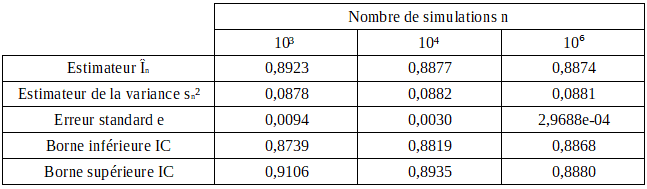
\includegraphics{Tableau_4.PNG}

\bigbreak
\bigbreak

\item La variance de la méthode de Monte Carlo avec variables de contrôle est plus petite que celle de la méthode avec échantillonnage préférentiel ainsi que de la première méthode. La méthode avec variable de contrôles est donc la meilleure des trois qui ont été vues pour le moment.\\
On remarque également sur le graphe de cette méthode (cf. \textbf{Annexe D - page 3}) que la vitesse de convergence est meilleure que celle des deux premières méthodes.

\end{questions}

\end{exercice}


\bigbreak
\bigbreak
\bigbreak

\subsection{Variables antithétiques}

\bigbreak


\noindent Soit $G$ une variable aléatoire gaussienne centrée et réduite. Comme $G$ et $-G$ ont la même loi, on peut approcher $C$ par $C \approx \frac{1}{2n} \sum_{i=1}^{n} \left[ \left( \text{e}^{G_{i}} - 1 \right)_{+} + \left( \text{e}^{-G_{i}} - 1 \right)_{+} \right]$, où $(G_{i})_{i \geq 1}$ est une suite de v.a.i.i.d. de loi gaussienne centrée et réduite.

\begin{questions}

\bigbreak

\item Justifions que l'on peut approcher $C$ par la quantité donnée dans l'énoncé ci-dessus.\\
\\

Posons $(Y_{i})_{i \geq 1} := \left( \frac{1}{2} \left[ \left( \text{e}^{G_{i}} - 1 \right)_{+} + \left( \text{e}^{-G_{i}} - 1 \right)_{+} \right] \right)_{i \geq 1}$. $(Y_{i})_{i \geq 1}$ est une suite de v.a.i.i.d de même loi que $Y_{1} = \frac{1}{2} \left[ \left( \text{e}^{G_{1}} - 1 \right)_{+} + \left( \text{e}^{-G_{1}} - 1 \right)_{+} \right]$ car les $G_{i}$ sont des v.a.i.i.d (de loi normale centrée réduite).\\
\\ 

On observe que : 

\begin{align*}
    \mathbb{E} [Y_{1}] &= \frac{1}{2} \left[ \mathbb{E} \left[ \left( \text{e}^{G_{1}} - 1 \right)_{+} \right] + \mathbb{E} \left[ \left( \text{e}^{-G_{1}} - 1 \right)_{+} \right] \right]\\
    &= \frac{1}{2} \left[ 2 \mathbb{E} \left[ \left( \text{e}^{G_{1}} - 1 \right)_{+} \right] \right] \ \ \ \ \text{car $G_{1}$ et $-G_{1}$ ont la même loi et donc $\mathbb{E} \left[\left( \text{e}^{G_{1}} - 1 \right)_{+} \right] = \mathbb{E} \left[\left( \text{e}^{-G_{1}} - 1 \right)_{+} \right]$}\\
    &= \mathbb{E} \left[\left( \text{e}^{G_{1}} - 1 \right)_{+} \right]\\
    &= C \ \ \ \ \text{par définition de $C$.}
\end{align*}

Ainsi, on introduit naturellement l'estimateur suivant :

\[\hat{I}_{n} = \frac{1}{n} \sum_{i=1}^{n} Y_{i} = \frac{1}{n} \sum_{i=1}^{n} \frac{1}{2} \left[ \left( \text{e}^{G_{i}} - 1 \right)_{+} + \left( \text{e}^{-G_{i}} - 1 \right)_{+} \right] =  \frac{1}{2n} \sum_{i=1}^{n} \left[ \left( \text{e}^{G_{i}} - 1 \right)_{+} + \left( \text{e}^{-G_{i}} - 1 \right)_{+} \right],\]

où $n \in \mathbb{N}^{*}$ correspond au nombre de simulations. Et on retrouve bien la quantité de l'énoncé.\\

Commme $\mathbb{E} [\hat{I}_{n}] = \frac{1}{n}  \sum_{i=1}^{n} \frac{1}{2} \left( \mathbb{E} \left[  \left( \text{e}^{G_{i}} - 1 \right)_{+} \right] + \mathbb{E} \left[ \left( \text{e}^{-G_{i}} - 1 \right)_{+} \right] \right) = \frac{1}{n} \times nC = C$, l'estimateur est sans biais.\\
\\

D'après la section 2.1 - point 1., on a que $\mathbb{E} [Y_{1} ] < \infty$. Ainsi, en appliquant la loi forte des grands nombres on déduit :

\[\underset{n \to \infty}{\text{lim}} \hat{I}_{n} = \underset{n \to \infty}{\text{lim}} \frac{1}{n} \sum_{i=1}^{n} \frac{1}{2} \left[ \left( \text{e}^{G_{i}}-1 \right)_{+} + \left( \text{e}^{-G_{i}}-1\right)_{+} \right] = C \ \ \text{p.s et dans $L^{1}$}.\]

Montrons que les $(Y_{i})_{i \geq 1}$ admettent un moment d'ordre $2$ afin de pouvoir appliquer le théorème central limite.\\
On montre donc que $\mathbb{E}[Y_{1}^{2}] < + \infty$. En appliquant le théorème de transfert,

\[\mathbb{E}[Y_{1}^{2}] = \mathbb{E} \left[\left( \frac{1}{2} \left[ \left( \text{e}^{G_{1}}-1 \right)_{+} + \left( \text{e}^{-G_{1}}-1 \right)_{+} \right] \right)^{2}  \right] = \frac{1}{4} \int_{\mathbb{R}} \left( \left(\text{e}^{x}-1 \right)_{+} + \left(\text{e}^{-x}-1 \right)_{+} \right)^{2} \times \frac{\text{e}^{-\frac{x^{2}}{2}}}{\sqrt{2\pi}}dx.\]

On a :


\begin{align*}
    \text{e}^{x}-1 \ \geq \ 0 \ &\Leftrightarrow \ \text{e}^{x} \geq 1\\
    &\Leftrightarrow \ x \ \geq \ 0,
\end{align*}

et : 

\begin{align*}
    \text{e}^{-x}-1 \ \geq \ 0 \ &\Leftrightarrow \ \text{e}^{-x} \geq 1\\
    &\Leftrightarrow \ -x \ \geq \ 0\\
    &\Leftrightarrow \ x \ \leq \ 0.
\end{align*}

Ainsi, 

\begin{align*}
    \mathbb{E}\left[ Y_{1}^{2} \right] &= \frac{1}{4} \left( \int_{-\infty}^{0} \left(\text{e}^{-x}-1\right)^{2} \times \frac{e^{-\frac{x^{2}}{2}}}{\sqrt{2\pi}}dx + \int_{0}^{+\infty} \left(\text{e}^{x}-1\right)^{2} \times \frac{e^{-\frac{x^{2}}{2}}}{\sqrt{2\pi}}dx \right)
\end{align*}

Posons : 

\[\left\{
  \begin{array}{lll}
    I_{1} := \int_{-\infty}^{0} \left(\text{e}^{-x}-1\right)^{2} \times \frac{e^{-\frac{x^{2}}{2}}}{\sqrt{2\pi}}dx\\
    I_{2} := \int_{0}^{+\infty} \left(\text{e}^{x}-1\right)^{2} \times \frac{e^{-\frac{x^{2}}{2}}}{\sqrt{2\pi}}dx,
\end{array}
\right.\]

de tel sorte qu'on ait : $\mathbb{E}\left[ Y_{1}^{2} \right] = \frac{1}{4} \left( I_{1}+I_{2} \right)$.\\
\\
\begin{itemize}
    \item \underline{Calcul de $I_{1}$ :}\\
    
    On fait un changement de variable : on pose $y:=-x$, donc $dy=-dx$.\\
    \\
Donc, 

\begin{align*}
    I_{1} &= \int_{0}^{+\infty} \left(\text{e}^{y}-1\right)^{2} \frac{\text{e}^{-\frac{y^{2}}{2}}}{\sqrt{2\pi}}dy
\end{align*}

D'après le point 1. de la section 2.2, on a que $I_{1} = \text{e}^{2}\phi(-2) -2\text{e}^{\frac{1}{2}}\phi(-1) + \phi(0)$.\\
\\

\item \underline{Calcul de $I_{2}$ :}\\

On remarque que $I_{2} = I_{1}$.
\end{itemize}

\bigbreak

Finalement, on a : 

\begin{align*}
    \mathbb{E}\left[ Y_{1}^{2} \right] &= \frac{1}{4} \left( I_{1} + I_{2} \right)\\
    &= \frac{1}{4} \left( 2I_{1} \right)\\
    &= \frac{1}{2} \left( I_{1} \right)\\
    &= \frac{1}{2} \left( \text{e}^{2} \phi(-2) -2\text{e}^{\frac{1}{2}} \phi(-1) + \phi(0) \right).
\end{align*}

Donc $\mathbb{E}\left[ Y_{1}^{2} \right] < \infty$ et les $(Y_{i})_{i \geq 1}$ admettent un moment d'ordre 2.\\

On pose $\sigma^{2} := Var(Y_{1}) = \mathbb{E}\left[ Y_{1}^{2} \right] - C^{2}$.\\
On a donc :

\begin{align*}
\sigma^{2} &= \frac{1}{2} \left( \text{e}^{2} \phi(-2) -2\text{e}^{\frac{1}{2}} \phi(-1) + \phi(0) \right) - \left( \text{e}^{\frac{1}{2}} \times 0,8413 - \frac{1}{2} \right)^{2}\\
&= \frac{1}{2} \left( \text{e}^{2} N(2) -2\text{e}^{\frac{1}{2}} N(1) + \frac{1}{2} \right) - \left( \text{e}^{\frac{1}{2}} \times 0,8413 - \frac{1}{2} \right)^{2}
\end{align*}

Et en remplaçant par les valeurs de $N(0)$, $N(1)$ et $N(2)$, on obtient :\\ 

\hspace{6.5cm}\fcolorbox{red}{white}{$\sigma^{2} \approx 1,6863$.}\\

La variance de la méthode de la section 2.2 - point 1. était égale à $4,1596$. 
Pour que la méthode des variables antithétiques soit intéressante, il faut que $\sigma^{2} < \frac{1}{2} \times 4,1596 = 2,0798$. Or, on a $\sigma^{2} \approx 1,6863 < 2,0798$. Donc la méthode des variables antithétiques est intéressante à effectuer et la variance est bien réduite. 

\bigbreak

On a que :

\[\text{Var}(\hat{I}_{n}) = \frac{\sigma^{2}}{n}.\]

L'application du théorème central limite implique que, lorsque $n$ tend vers l'infini, 

\[\frac{\sqrt{n}}{\sigma}(\hat{I}_{n} - C) \ \ \text{converge en loi vers $\mathcal{N}(0,1)$,}\]

On remplace $\sigma^{2}$ par l'estimateur classique de la variance : 

\[s_{n}^{2} = \frac{1}{n-1} \sum_{i=1}^{n} \left( Y_{i} - \hat{I}_{n} \right)^{2} = \frac{1}{n-1} \left( \sum_{i=1}^{n} Y_{i}^{2} - n\hat{I}_{n}^{2} \right).\]

On utilise les approximations suivantes :\\
\\
\textit{Erreur standard} : $\frac{\sigma}{\sqrt{n}} \approx \frac{s_{n}}{\sqrt{n}}$\\
\textit{Erreur relative} : $\frac{1}{C}\frac{\sigma}{\sqrt{n}} \approx \frac{1}{\hat{I}_{n}}\frac{s_{n}}{\sqrt{n}}$.\\
\\

On décide de choisir un intervalle de confiance au niveau $\alpha = 95 \ \%$. Ainsi, l'intervalle de confiance de $C$ au nivau $95 \ \%$ est :

\[ \left[ \hat{I}_{n} - 1.96 \frac{s_{n}}{\sqrt{n}}, \hat{I}_{n} + 1.96 \frac{s_{n}}{\sqrt{n}} \right].\]


\bigbreak
\bigbreak

\item \underline{\textbf{Algorithme de Monte Carlo :}}\\

On peut écrire un algorithme de Monte Carlo car les hypothèses sont vérifiées (en particulier $\mathbb{E} [Y_{1}^{2} ] < \infty)$. Le code Matlab de l'algorithme de Monte Carlo associé à ce point ainsi que le graphique correspondant et les valeurs que nous renvoie le programme est consultable en \textbf{Annexe E}.\\

J'ai exécuté le programme pour différentes valeurs de $n$ : \\

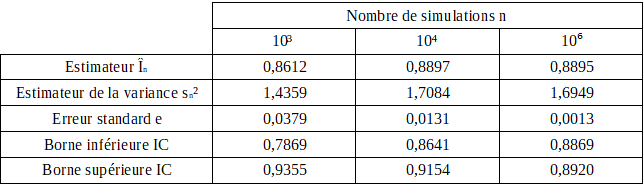
\includegraphics{Tableau_5.PNG}

La variance de l'estimateur est donnée par $\text{Var}(\hat{I}_{n}) = \frac{\sigma^{2}}{n}$.\\

\underline{Pour $n=10^{4}$ :}\\

$\text{Var}(\hat{I}_{n}) = \frac{1,6863}{10^{4}} \approx 1,6863\times 10^{-4}$ et la valeur approchée de l'estimateur est : $0,8897$.
    
    

\bigbreak
\bigbreak

\item La variance de la méthode avec variables antithétiques est plus petite que la variance de la première méthode mais plus grande que celle de toutes les autres. Cette méthode semble converger à partir d'environ $3000$ simulations (d'après le graphe de cette méthode - cf. \textbf{Annexe E - page 3}), ce qui est toujours mieux que la méthode de la section 2.1 mais évidemment moins bien que celle de la section 2.3 (cf. \textbf{Annexe C - page 3}) ou 2.4 (cf. \textbf{Annexe D - page 3}).

\end{questions}

\end{exercice}

\bigbreak
\bigbreak
\bigbreak

\subsection{Comparaison}



\begin{questions}

\item Présentons les résulats que l'on a obtenu à travers les différentes méthodes de Monte Carlo pour le calcul de $C$ utilisées dans ce projet. On présentera nos résultats pour $n=10^{3}$, $n=10^{4}$ et $n=10^{6}$.\\

\underline{\textbf{Tableau récapitulatif :}}\\

\hspace{-2.85cm}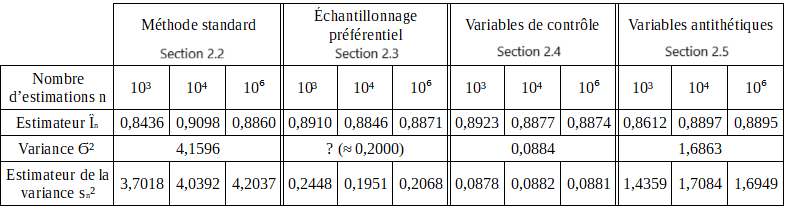
\includegraphics{Tableau_6bis.png}

\bigbreak
\bigbreak

\item On voit clairement que la méthode ayant la plus petite variance est la méthode de Monte Carlo avec variables de contrôle de la section 2.4. Cette méthode est donc la meilleure de celles étudiées. On remarque également que la valeur de l'estimateur de C : $\hat{I}_{n}$ est très proche de la valeur théorique de $C$ (qui est égale à $0,8871$) pour la méthode avec variables de contrôle, que ce soit aussi bien pour $n=10^{3}$, $n=10^{4}$ ou encore $n=10^{6}$.\\
La précision des méthodes des sections 2.3 et 2.5 semblent plutôt bonnes aussi mais c'est surtout dans la première méthode de Monte Carlo (celle de la section 2.2) que l'on observe une précision un peu plus médiocre.



\end{questions}

\end{exercice}

\bigbreak
\bigbreak

\noindent\underline{Remarque concernant tout le projet :} Pour chaque section, on a remplacé la variance $\sigma^{2}$ par l'estimateur $s_{n}^{2}$. Or, comme on connaît la variance théorique $\sigma^{2}$ dans chaque section (sauf la section 2.3 où je n'ai pas réussi à la déterminer), il aurait été sûrement plus judicieux de conserver $\sigma^{2}$ pour nos méthodes de Monte Carlo, quitte à remplacer $\sigma^{2}$ par l'estimateur $s_{n}^{2}$ là où on n'arrive pas à calculer $\sigma^{2}$, comme dans la section 2.3.



\section{Conclusion}

\noindent Finalement, parmi les $4$ méthodes de Monte-Carlo que l'on a élaboré, nous avons réussi à en déterminer une meilleure que les autres. Cette méthode se trouve être celle avec variables de contrôle, qui est une méthode de réduction de variance. Pour comparer les différentes méthodes entre elles, on a regardé principalement leur variance respective puis on a comparé les variances : plus la variance de la méthode est petite et plus cette méthode est efficace. \\
De plus, on remarque que les méthodes de Monte-Carlo avec réduction de variance (dans ce projet ce sont celles des sections 2.3, 2.4 et 2.5) semblent assez précises dans l'estimation de $C$ ou $P$, surtout quand le nombre de simulations est grand ($n=10^{4}$, $n=10^{6}$).


\newpage

\begin{appendices}

\setcounter{page}{1}
\section{Annexe A : Table de la loi Normale centrée réduite}

\bigbreak
\bigbreak

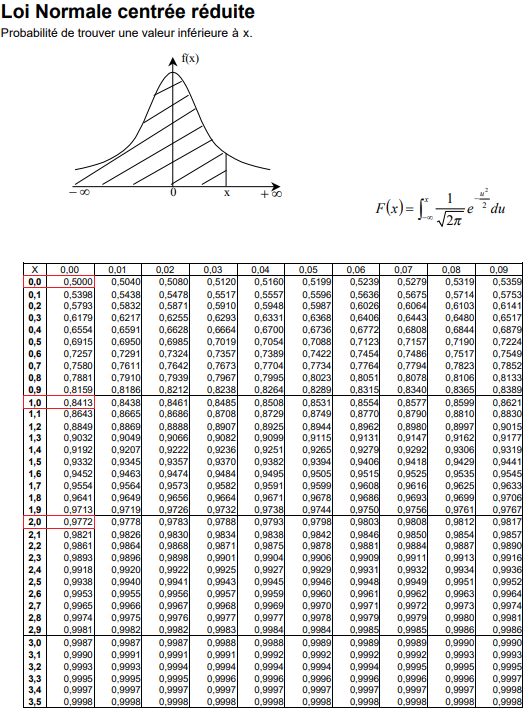
\includegraphics{Normal_Distribution_Table.png}

\end{appendices}


\newpage


\begin{appendices}

\setcounter{page}{1}
\section{Annexe B : Code Matlab et graphique de la section 2.2}

\bigbreak
\bigbreak

\hspace{-2.4cm}\underline{Algorithme de Monte Carlo de la section 2.2 - point 1. (pour le call) :}\\

\hspace{-2.5cm}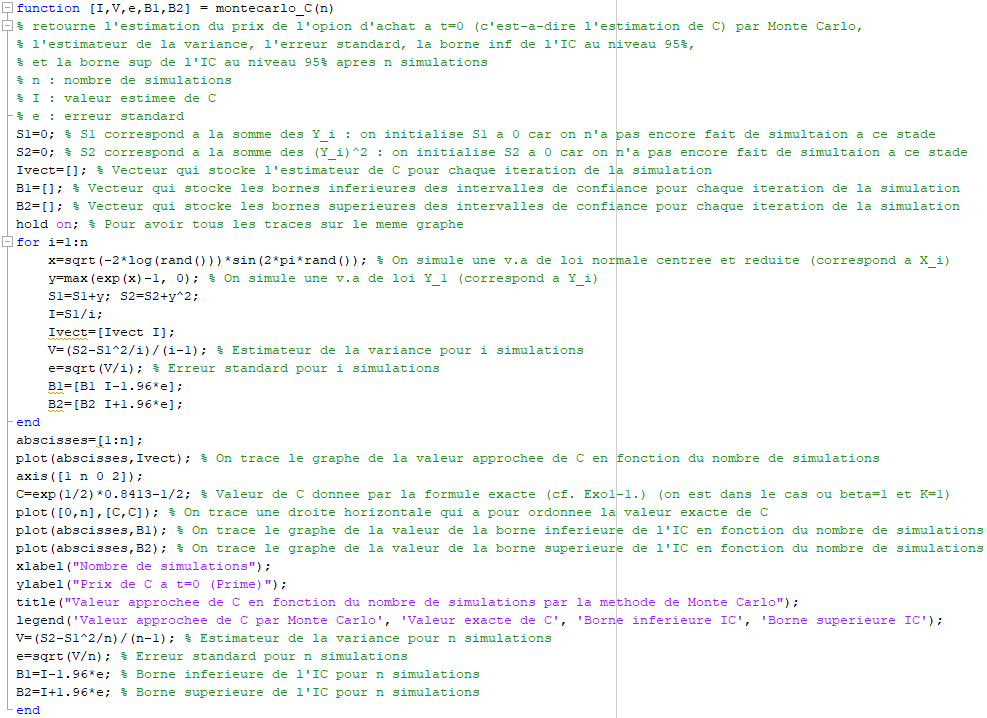
\includegraphics[scale=0.80]{montecarlo_C.PNG}

\newpage

\underline{Ce que retourne l'algorithme montecarlo\_C pour $n = 10^{3}$, $n = 10^{4}$ et $n = 10^{6}$ :}

\begin{figure}[h]
    \begin{minipage}[c]{.46\linewidth}
        \centering
        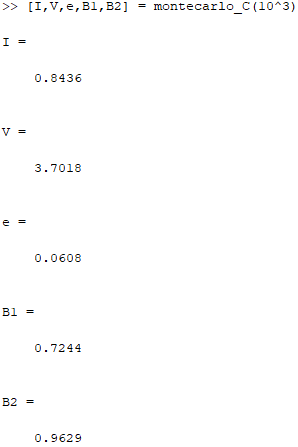
\includegraphics[scale=0.80]{return1_montecarlo_C.PNG}
    \end{minipage}
    \hfill
    \begin{minipage}[c]{.46\linewidth}
        \centering
        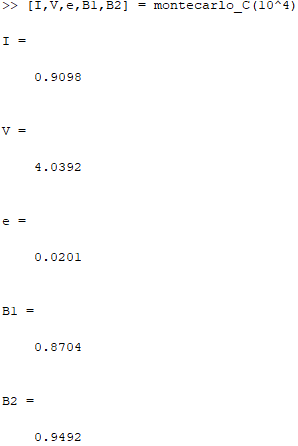
\includegraphics[scale=0.80]{return2_montecarlo_C.PNG}
    \end{minipage}
\end{figure}


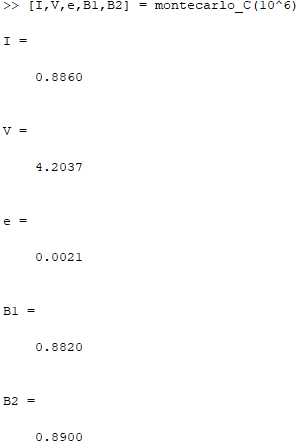
\includegraphics[scale=0.80]{return3_montecarlo_C.PNG}

\newpage

\hspace{-1.7cm}\underline{Graphique tracé par l'algorithme montecarlo\_C pour $n=10^{4}$:}\\

\hspace{-1.7cm}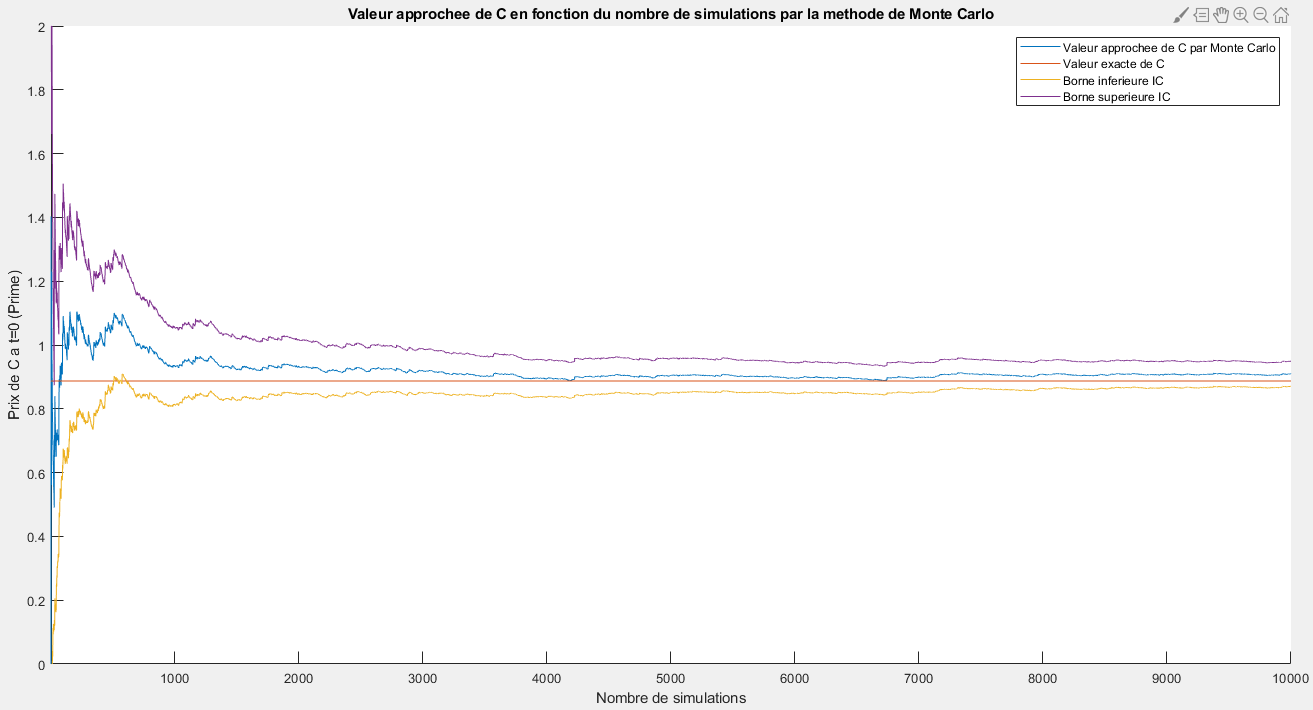
\includegraphics[scale=0.55]{graphe_montecarlo_C.PNG}

\newpage

\hspace{-2.4cm}\underline{Algorithme de Monte Carlo de la section 2.2 - point 2. (pour le put) :}\\

\hspace{-2.5cm}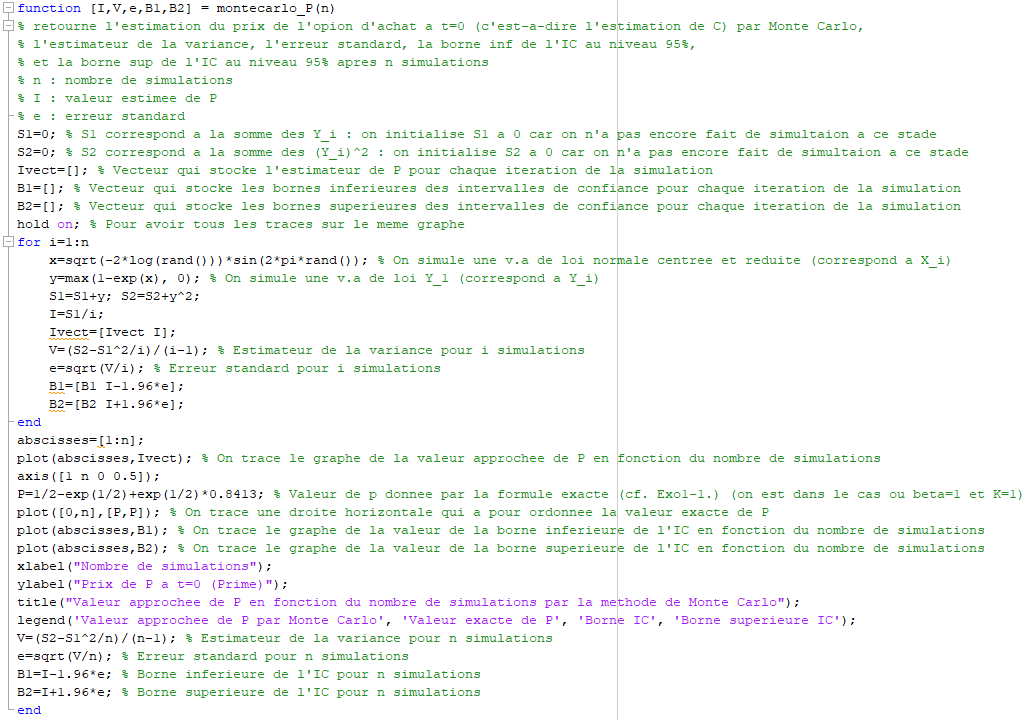
\includegraphics[scale=0.80]{montecarlo_P.PNG}\\


\hspace{-2.4cm}\underline{Remarque :} Une petite partie du code est rognée mais c'est écrit la même chose que dans l'algorithme du point 1. de la section 2.1. : << (on est dans le cas où beta=1 et K=1) >>.

\newpage

\underline{Ce que retourne l'algorithme montecarlo\_P pour $n = 10^{3}$, $n = 10^{4}$ et $n = 10^{6}$ :}

\begin{figure}[h]
    \begin{minipage}[c]{.46\linewidth}
        \centering
        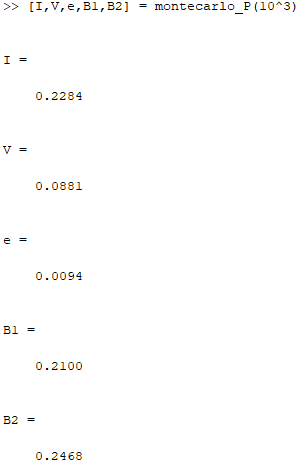
\includegraphics[scale=0.80]{return1_montecarlo_P.PNG}
    \end{minipage}
    \hfill
    \begin{minipage}[c]{.46\linewidth}
        \centering
        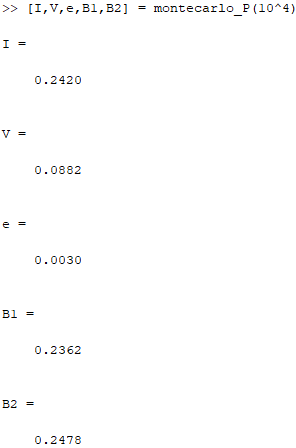
\includegraphics[scale=0.80]{return2_montecarlo_P.PNG}
    \end{minipage}
\end{figure}


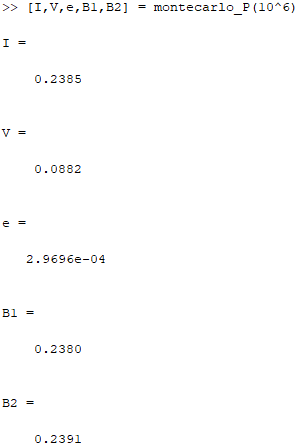
\includegraphics[scale=0.80]{return3_montecarlo_P.PNG}

\newpage

\hspace{-1.7cm}\underline{Graphique tracé par l'algorithme montecarlo\_P pour $n=10^{4}$:}\\

\hspace{-1.7cm}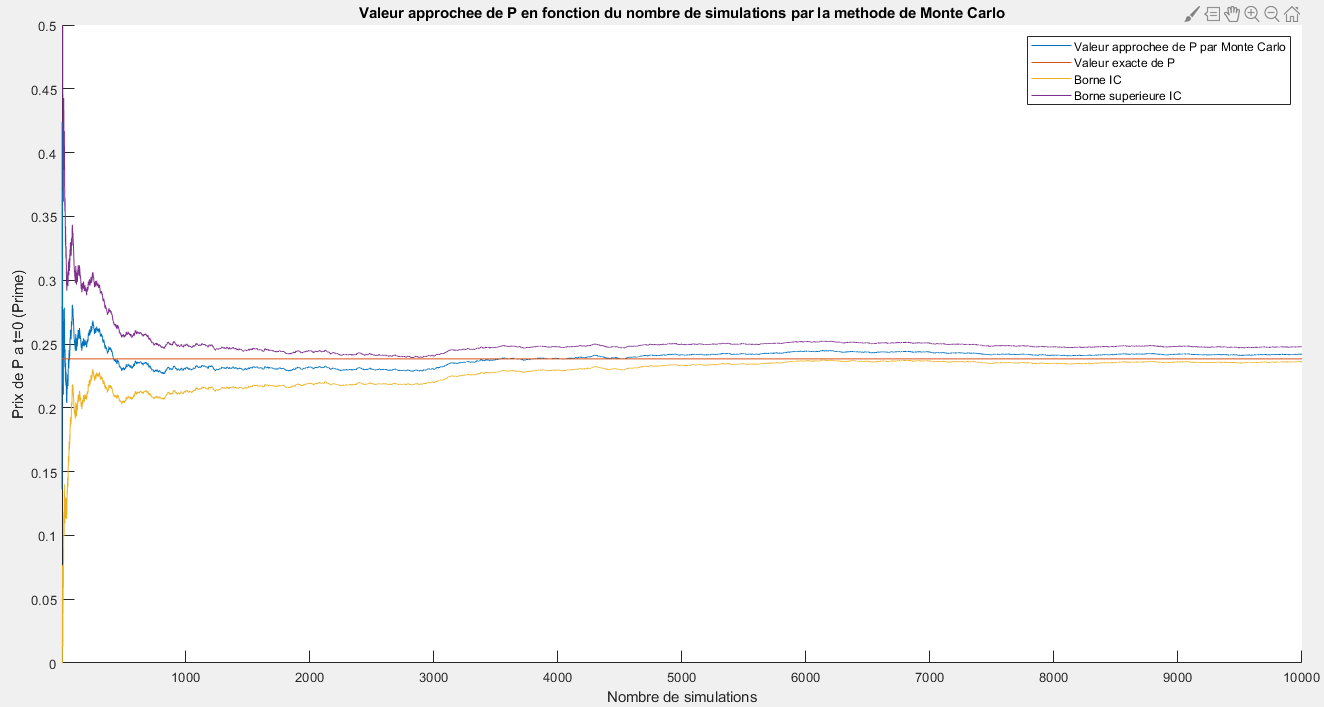
\includegraphics[scale=0.55]{graphe_montecarlo_P.PNG}

\end{appendices}


\newpage


\begin{appendices}

\setcounter{page}{1}
\section{Annexe C : Code Matlab et graphique de la section 2.3}

\bigbreak
\bigbreak

\hspace{-2.4cm}\underline{Algorithme de Monte Carlo de la section 2.3 :}\\

\hspace{-2.5cm}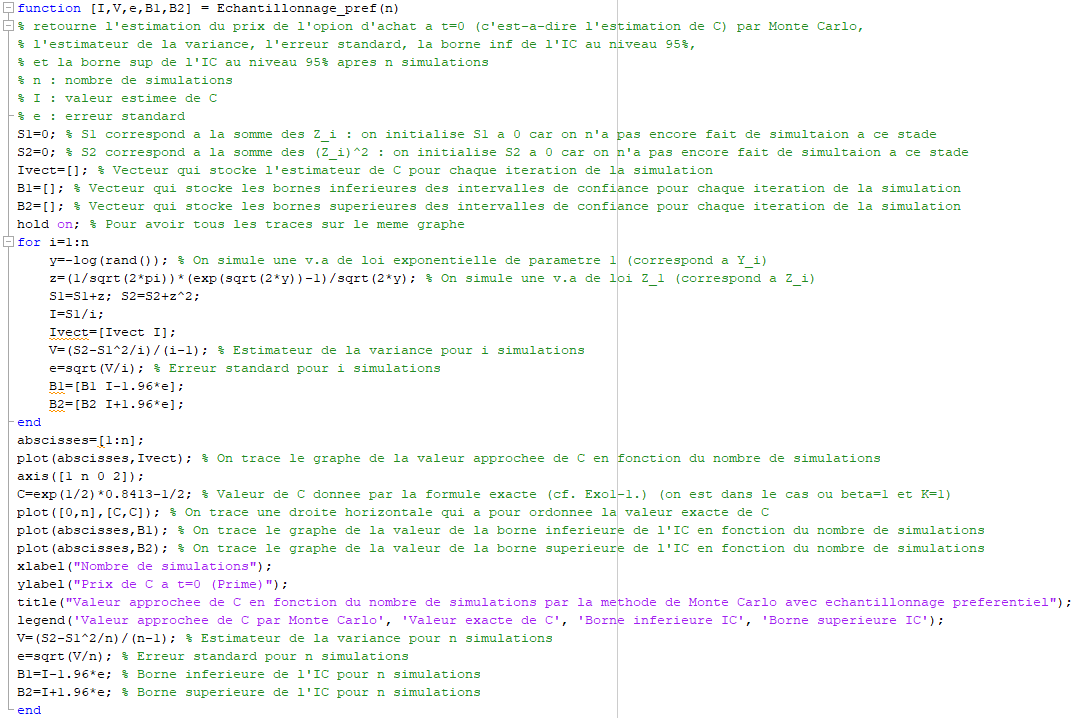
\includegraphics[scale=0.80]{Echantillonnage_pref.PNG}\\

\hspace{-2.4cm}\underline{Remarque :} Une petite partie du code est rognée à la fin. C'est écrit : << avec echantillonnage preferentiel"); >>.

\newpage

\underline{Ce que retourne l'algorithme Echantillonnage\_pref pour $n = 10^{3}$, $n = 10^{4}$ et $n = 10^{6}$ :}

\begin{figure}[h]
    \begin{minipage}[c]{.46\linewidth}
        \centering
        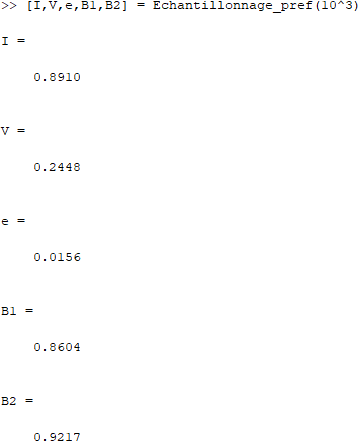
\includegraphics[scale=0.80]{return1_Echantillonnage_pref.PNG}
    \end{minipage}
    \hfill
    \begin{minipage}[c]{.46\linewidth}
        \centering
        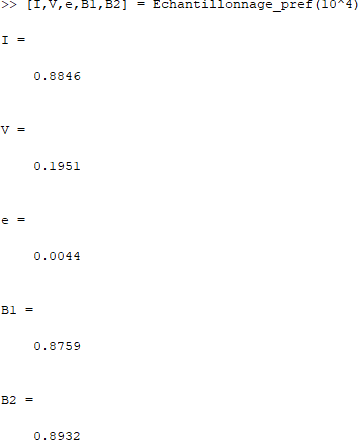
\includegraphics[scale=0.80]{return2_Echantillonnage_pref.PNG}
    \end{minipage}
\end{figure}


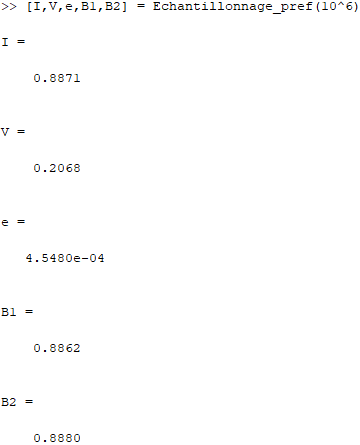
\includegraphics[scale=0.80]{return3_Echantillonnage_pref.PNG}

\newpage

\hspace{-1.7cm}\underline{Graphique tracé par l'algorithme Echantillonnage\_pref pour $n=10^{4}$:}\\

\hspace{-1.7cm}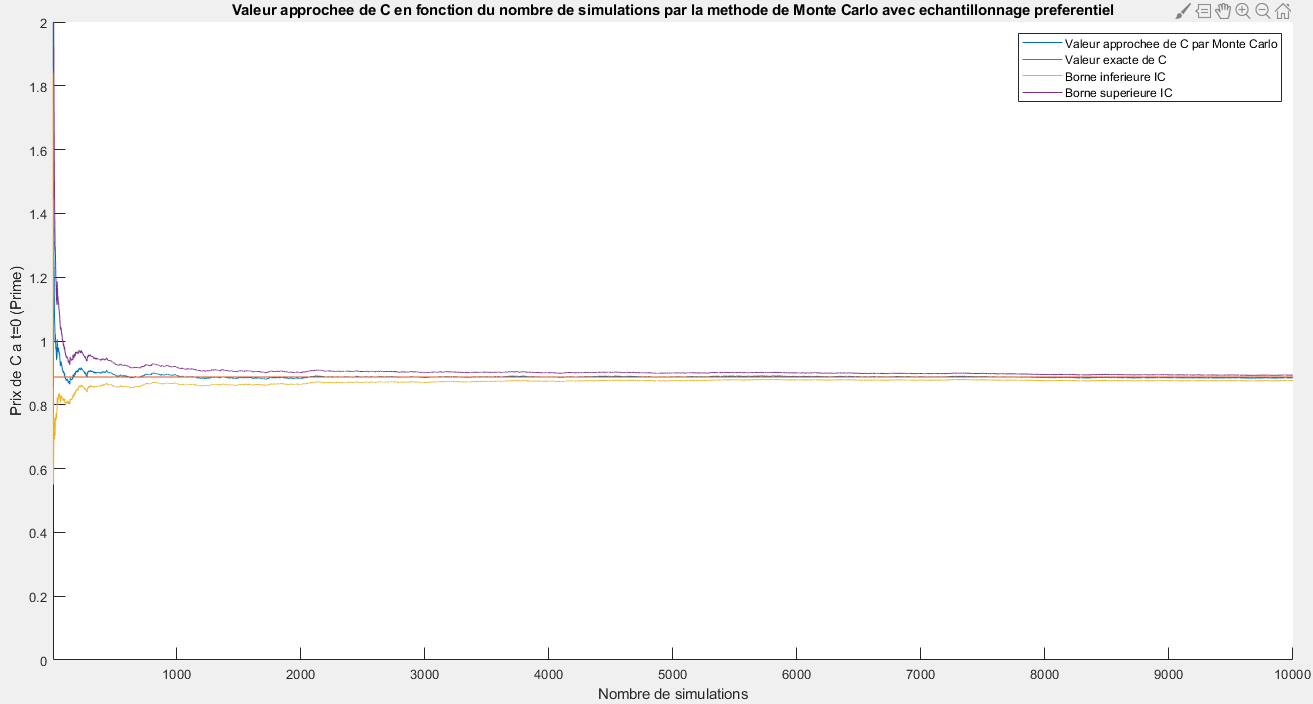
\includegraphics[scale=0.55]{graphe_Echantillonnage_pref.PNG}

\end{appendices}


\newpage

\begin{appendices}

\setcounter{page}{1}
\section{Annexe D : Code Matlab et graphique de la section 2.4}

\bigbreak
\bigbreak

\hspace{-2.4cm}\underline{Algorithme de Monte Carlo de la section 2.4 :}\\

\hspace{-2.5cm}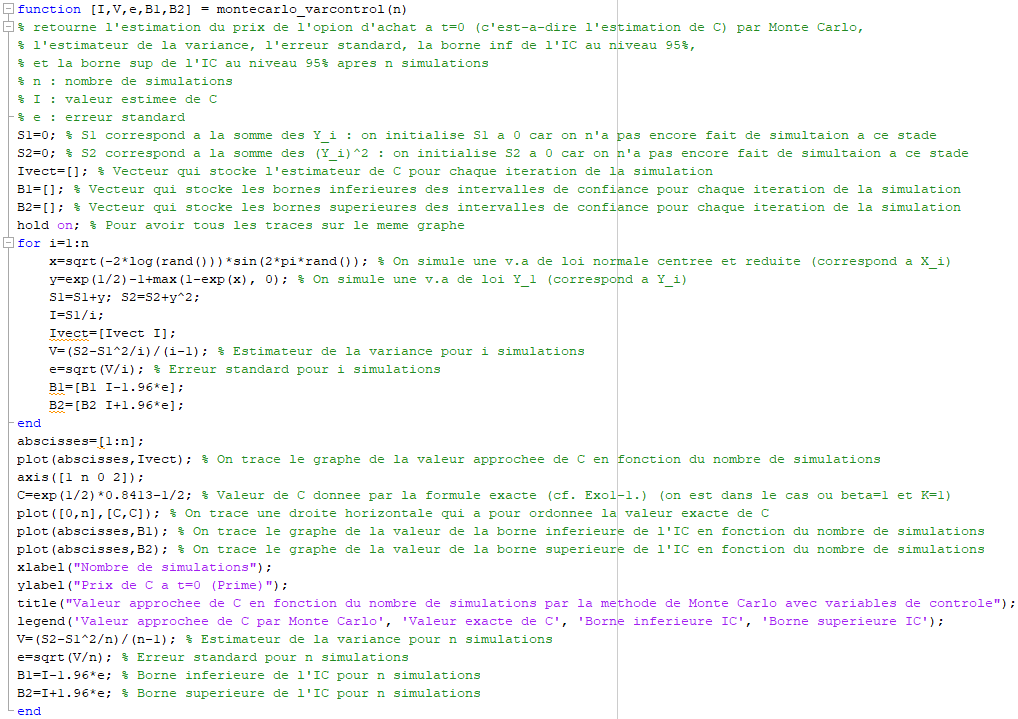
\includegraphics[scale=0.80]{montecarlo_varcontrol.PNG}\\

\hspace{-2.4cm}\underline{Remarque :} Une petite partie du code est rognée à la fin. C'est écrit : << avec variables de controle"); >>.

\newpage

\underline{Ce que retourne l'algorithme montecarlo\_varcontrol pour $n = 10^{3}$, $n = 10^{4}$ et $n = 10^{6}$ :}

\begin{figure}[h]
    \begin{minipage}[c]{.46\linewidth}
        \centering
        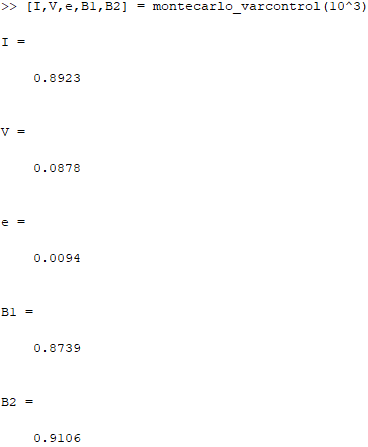
\includegraphics[scale=0.80]{return1_montecarlo_varcontrol.PNG}
    \end{minipage}
    \hfill
    \begin{minipage}[c]{.46\linewidth}
        \centering
        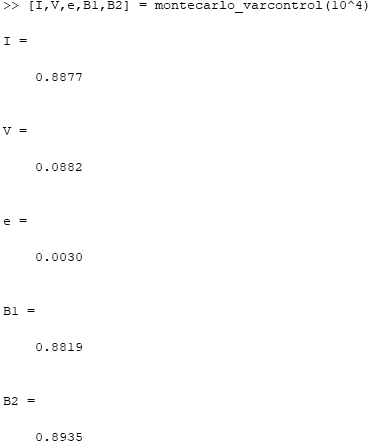
\includegraphics[scale=0.80]{return2_montecarlo_varcontrol.PNG}
    \end{minipage}
\end{figure}


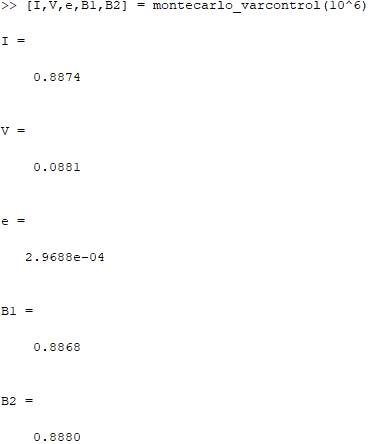
\includegraphics[scale=0.80]{return3_montecarlo_varcontrol.PNG}

\newpage

\hspace{-1.7cm}\underline{Graphique tracé par l'algorithme montecarlo\_varcontrol pour $n=10^{4}$:}\\

\hspace{-1.7cm}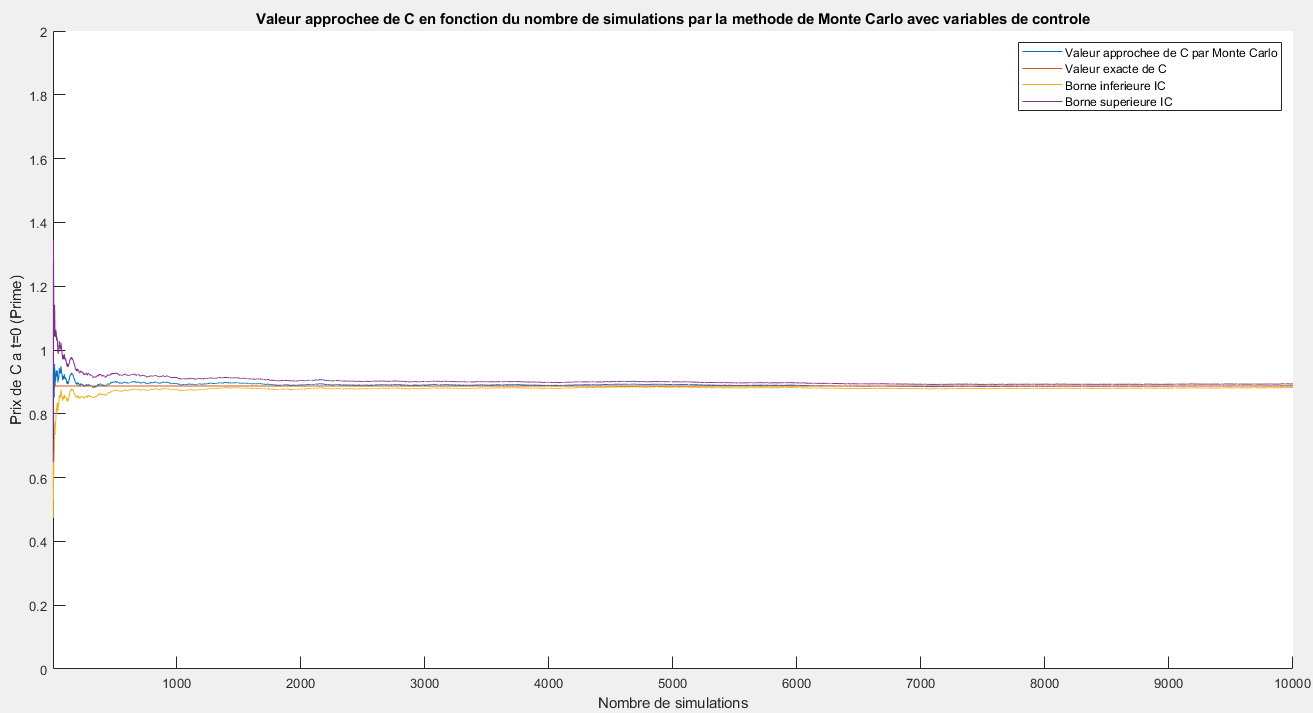
\includegraphics[scale=0.55]{graphe_montecarlo_varcontrol.PNG}
\end{appendices}


\newpage 


\begin{appendices}

\setcounter{page}{1}
\section{Annexe E : Codes Matlab et graphique de la section 2.5}

\bigbreak
\bigbreak

\hspace{-2.4cm}\underline{Algorithme de Monte Carlo de la section 2.5 :}\\

\hspace{-2.5cm}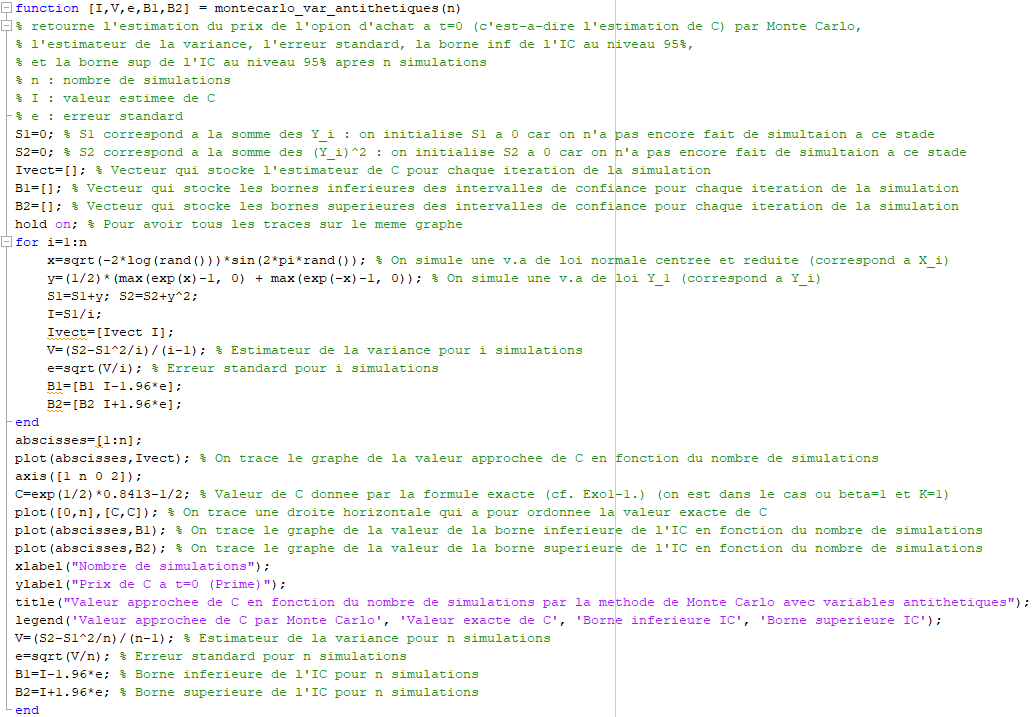
\includegraphics[scale=0.80]{montecarlo_var_antithetiques.PNG}\\

\hspace{-2.4cm}\underline{Remarque :} Une petite partie du code est rognée à la fin. C'est écrit : << avec variables antithetiques"); >>.

\newpage

\underline{Ce que retourne l'algorithme montecarlo\_var\_antithetiques pour $n = 10^{3}$, $n = 10^{4}$ et $n = 10^{6}$ :}

\begin{figure}[h]
    \begin{minipage}[c]{.46\linewidth}
        \centering
        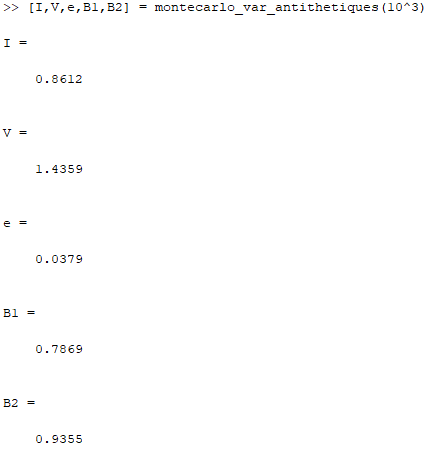
\includegraphics[scale=0.80]{return1_montecarlo_var_antithetiques.PNG}
    \end{minipage}
    \hfill
    \begin{minipage}[c]{.46\linewidth}
        \centering
        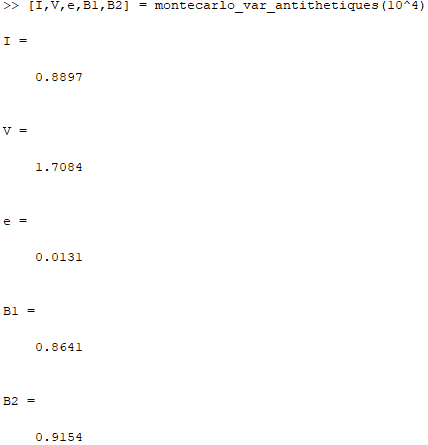
\includegraphics[scale=0.80]{return2_montecarlo_var_antithetiques.PNG}
    \end{minipage}
\end{figure}


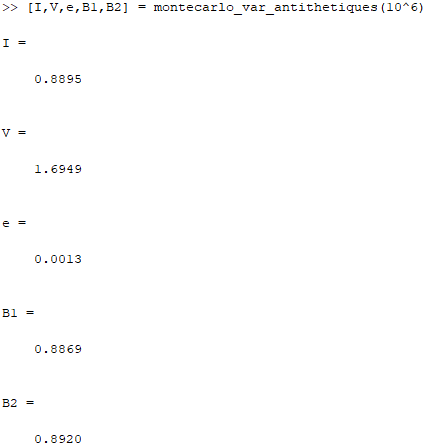
\includegraphics[scale=0.80]{return3_montecarlo_var_antithetiques.PNG}

\newpage

\hspace{-1.7cm}\underline{Graphique tracé par l'algorithme montecarlo\_var\_antithetiques pour $n=10^{4}$:}\\

\hspace{-1.7cm}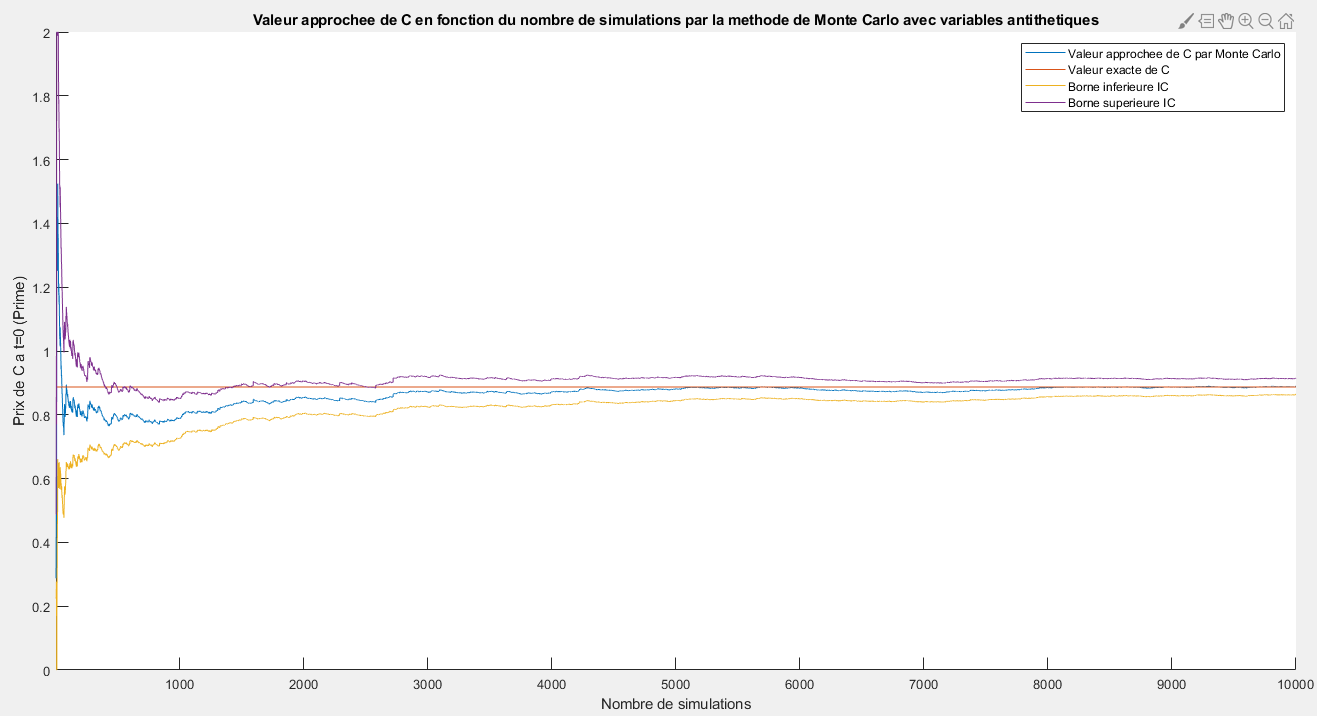
\includegraphics[scale=0.55]{graphe_montecarlo_var_antithetiques.PNG}

\end{appendices}

\end{document}